%%%%%%%%%%%%%%%%%%%%%%%%%%%%%%%%%%%%%%%%%%%%%%%%%%%%%%%%%%%%%%%%%%% 
%                                                                 %
%                            CHAPTER                              %
%                                                                 %
%%%%%%%%%%%%%%%%%%%%%%%%%%%%%%%%%%%%%%%%%%%%%%%%%%%%%%%%%%%%%%%%%%% 
\chapter{Results}
\label{chap:results}

\section{Setup}
A fully adjustable setup is created and used to generate three datasets with different lighting conditions.

The datasets are tested with the described program from \ref{sec:impl:visionalgorithms}. The results and graphs where obtained with Google Colab on a regular GPU, wandb was used for processing the logs.

The discussion is listed for every dataset starting with the second handmade dataset then the results of the Birthday dataset are listed. The Spaghetti dataset is listed third and finally the second handmade dataset is compared with the spaghetti dataset.

\section{Second handmade dataset results}
The second handmade dataset was created in section \ref{sec:impl:ds:shm}. An example of this dataset is given in Figure \ref{fig:res:shm:example}. For this dataset 905 test runs where conducted with different parameters to obtain the best possible results. First an overview is given on the overall performance by listing the five best runs. Next these results are compared for the different initialized model architectures as described in \ref{sec:impl:visionalgorithms:init}. The influences of parameters are discussed to conclude with a few example results on the test set.

\begin{figure}[hbtp]
\centering
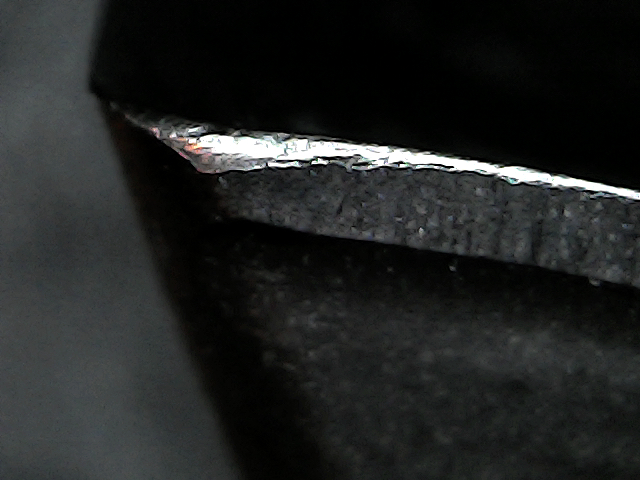
\includegraphics[width=.3\textwidth]{fig/Vision/Dataset/handmade_datasets/Second_handmade_dataset/b_003_p_004_s.jpg}
\caption{Example of second handmade dataset batch 3 insert 4.}
\label{fig:res:shm:example}
\end{figure}

\subsection{Overall results}


	For the five best runs we get up to a validation accuracy of 100\%, a test accuracy of 100\% and a train accuracy of 97\% as we can see on Figure \ref{fig:results:shm:overall}. This is almost a perfect result for the classification model. Bear in mind that this is just performed on 100 pictures separated in three categories: train, validation and test. These categories have 71, 20 and 9 pictures respectively. Since there are so little test pictures the test score is not fully valid but we can conclude this is a very good test run.

	\begin{figure}[hbtp]
		\begin{subfigure}{0.31\textwidth}
			\centering
			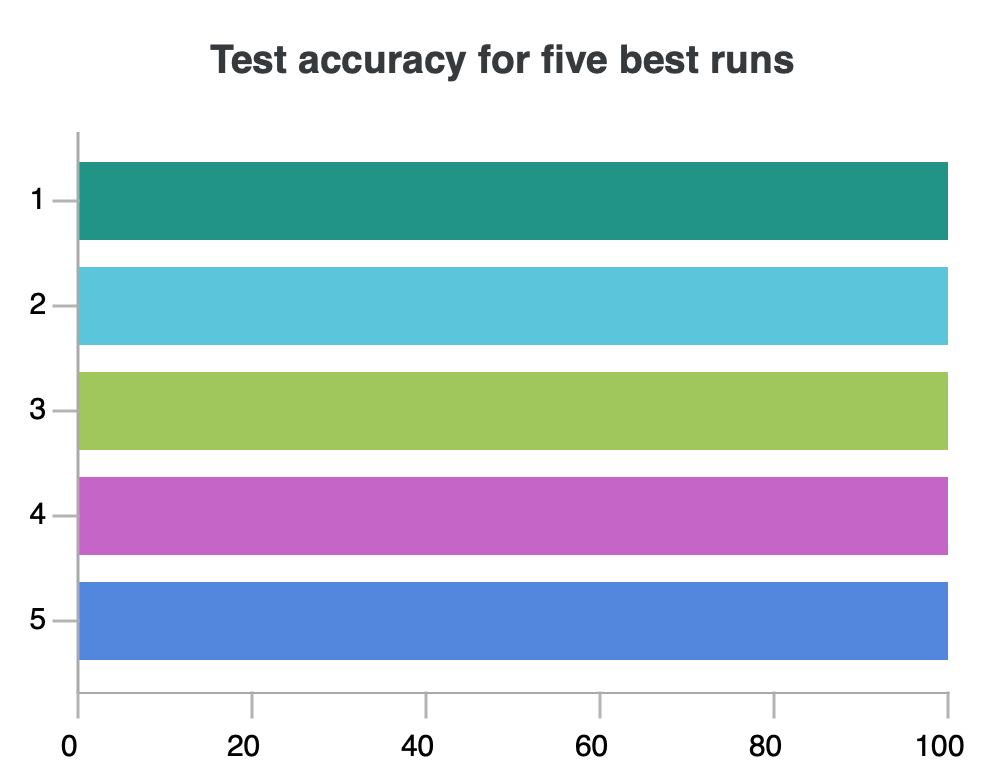
\includegraphics[width=\linewidth]{fig/results/wandb/second_handmade_sweep/charts/Section-2-Panel-0-jm7rxjojx.png}
			\caption{Test accuracy}
		\end{subfigure}
		\hspace*{\fill}   % maximizeseparation between the subfigures
		\begin{subfigure}{0.31\textwidth}
			\centering
			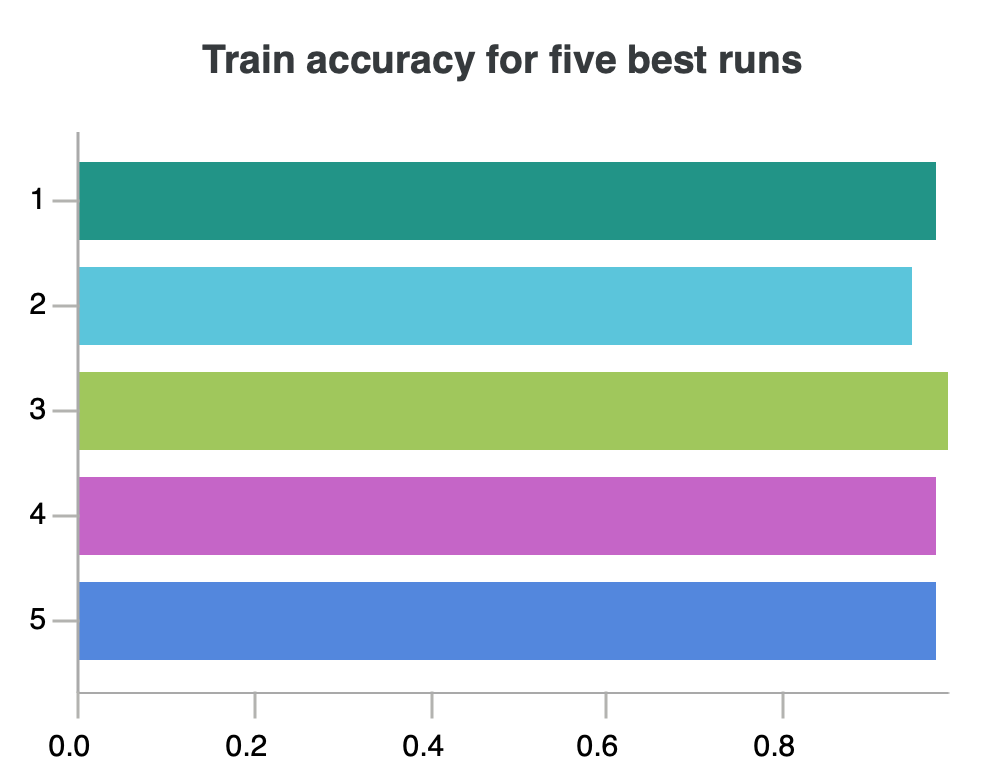
\includegraphics[width=\linewidth]{fig/results/wandb/second_handmade_sweep/charts/Section-2-Panel-1-mvdok5l4p.png}
			\caption{Train accuracy}
		\end{subfigure}
		\hspace*{\fill}   % maximizeseparation between the subfigures
		\begin{subfigure}{0.31\textwidth}
			\centering
			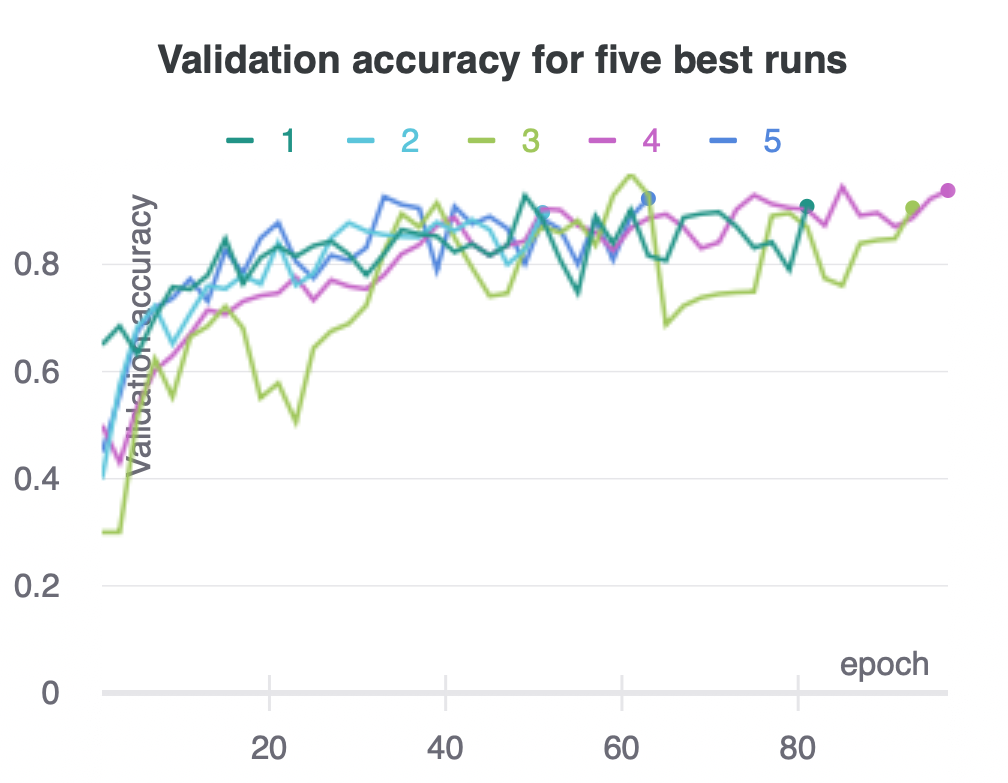
\includegraphics[width=\linewidth]{fig/results/wandb/second_handmade_sweep/charts/Section-2-Panel-2-p9dhpnuq6.png}
			\caption{Validation accuracy}
		\end{subfigure}
		\caption{Test, train and validation accuracy for five best runs with second handmade dataset.}
		\label{fig:results:shm:overall}
	\end{figure}

\subsection{Comparison between different model architectures}
	To get a better overview on how different architectures perform on the dataset, we compare the main results for all these tested architectures. Starting with Test accuracy on these models, later the validation accuracy is discussed.
	
	\subsubsection{Test accuracy}
	The test accuracy on 9 pictures from different classes that were randomly picked is really high. For 4 out of 5 model architectures the test accuracy is 100\% so all inserts where predicted correctly. Densenet is performing a little worse with an accuracy of 89\% what means that only one image wasn't predicted correctly. This is the result of testing 905 different parameters during training of the model. VGG11\_bn is showing a smaller difference between the minimum test accuracy of all tests and the maximum accuracy of all tests. For now the VGG11\_bn is the best model architecture based on the test accuracy.
	
	\begin{figure}[hbtp]
		\centering
		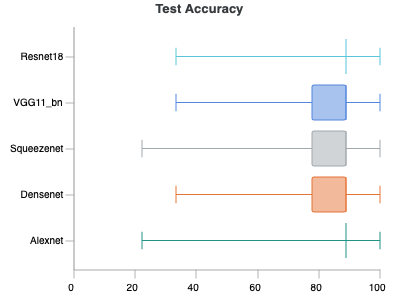
\includegraphics[width=0.49\textwidth]{fig/results/wandb/second_handmade_sweep/charts/test_accuracy_boxplot.png}
		\caption{Test accuracy for different model architectures with maximum and minimum values.}
	\end{figure}
	
	\begin{table}
	\centering
	\caption{Confusion matrix for tests of the second handmade dataset.}
		\begin{tabular}{ c c c c }
		%\caption{Confusion matrix for tests of Second handmade dataset}
						& Low 	& Medium & High	\\
		 Low 			& x 		& 2 			& 0		\\ 
		 Medium 	& 2 		& x 			& 5 		\\  
		 High 		& 0 		& 2 			& x   
		\end{tabular}
		\label{tab:results:shm:confusion}
		\end{table}
	
		A simple confusion matrix is created in table \ref{tab:results:shm:confusion} for 9 runs with 9 images each. Where the truth values are listed from top to bottom and the predicted values left to right.
	To interpret this table we look at the border between low and medium wear which is at 130 micrometer and the border between Medium and High wear at 230 micrometer. Since these limits are fixed numbers there are a lot of values just before and just after the limit. This makes it hard for the algorithm since it isn't even possible to see a difference between these images for the human eye. The confusion shows that the predictions between Medium and High are the most difficult. What we can also find is that there are no predictions totally wrong where High wear is predicted as low or vice versa.
	


	\subsubsection{Validation accuracy}
		The validation accuracy is plotted relative to the epochs in Figure \ref{fig:results:shm:validaccuracy} which gives an overview of how the training went. The beginning represents a learning curve which stabilises at the end of the graph. This means the training got a good amount of epochs to reach the optimal point of maximum validation accuracy.

		The graph is smoothed to create a better overview. The shadows behind are the standard deviation for each model. Some models tend to train faster to a higher validation accuracy like Alexnet and Squeezenet. However this doesn't result in a better outcome for Alexnet where the median scores worse. 

		Validation accuracy for best runs is given in table \ref{tab:results:shm:architectures:valacc}. There are two measurement values we can use namely the highest test accuracy and the highest validation accuracy. In the first column the highest reached validation accuracy is given for each model. We can see here that more models reach 100\% validation accuracy which should translate into a good generalisation. The results of the generalisation are given in the second column. Here the numbers represent the highest values for validation accuracy from the runs with the highest values for test accuracy. Or the table of all runs is sorted on test accuracy and the validation accuracy is taken from the first five runs. Here we can see the order isn't changed, there is just 5\% lost in accuracy. It declares the link between validation accuracy and test accuracy. 
		\begin{table}
		\caption{Best validation accuracy for different deep learning architectures. Sorted on best validation accuracy in column 1 and sorted on test accuracy in column 2.}
			\begin{tabular}{ c | c c }
			%\caption{Confusion matrix for tests of Second handmade dataset}
			Model name		& Validation Accuracy 	& Validation accuracy sorted on test accuracy	\\ \hline
		 	Alexnet 				& 100\%						& 100\% 				\\ 
		 	Resnet 18 			& 100\%						& 95\%					\\
		 	Squeezenet 		& 100\%						& 95\%					\\
		 	VGG11\_bn			& 95\%							& 90\%					\\
		 	Densenet			& 95\%							& 90\%					\\
			\end{tabular}
			\label{tab:results:shm:architectures:valacc}
		\end{table}

	\begin{figure}[hbtp]
		\centering
		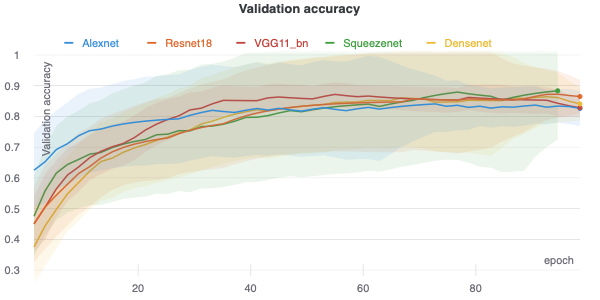
\includegraphics[width=0.6\textwidth]{fig/results/wandb/second_handmade_sweep/charts/valid_accuracy_median.png}
		\caption{Best validation accuracy for different model architectures.}
		\label{fig:results:shm:validaccuracy}
	\end{figure}

\subsection{Influence of Transfer learning on the results}
	The influence of transfer learning from the imagenet dataset is visualised in the graphs on Figure \ref{fig:res:shm:tl}. The test accuracy is plotted first for every model architecture and with transfer learning (TL) or without transfer learning (No TL) in Figure \ref{fig:res:shm:tl:ta}. It can be seen that the results are almost identical for the two different settings. The maximum test accuracy measured is 100\% for every model. The distributions changed a little bit which may be caused by the amount of test runs conducted for that specific model architecture.

The second graph on Figure \ref{fig:res:shm:tl:va} plots the validation accuracy for the different networks with and without transfer learning. From these boxplots we can see that Alexnet benefits from transfer learning. What would be due to the architectures small amount of parameters. Squeezenet and Resnet 18 actually get worse results with transfer learning opposed to traning without transfer learning.


\begin{figure}[hbtp]
	\begin{subfigure}{0.49\textwidth}
		\centering
		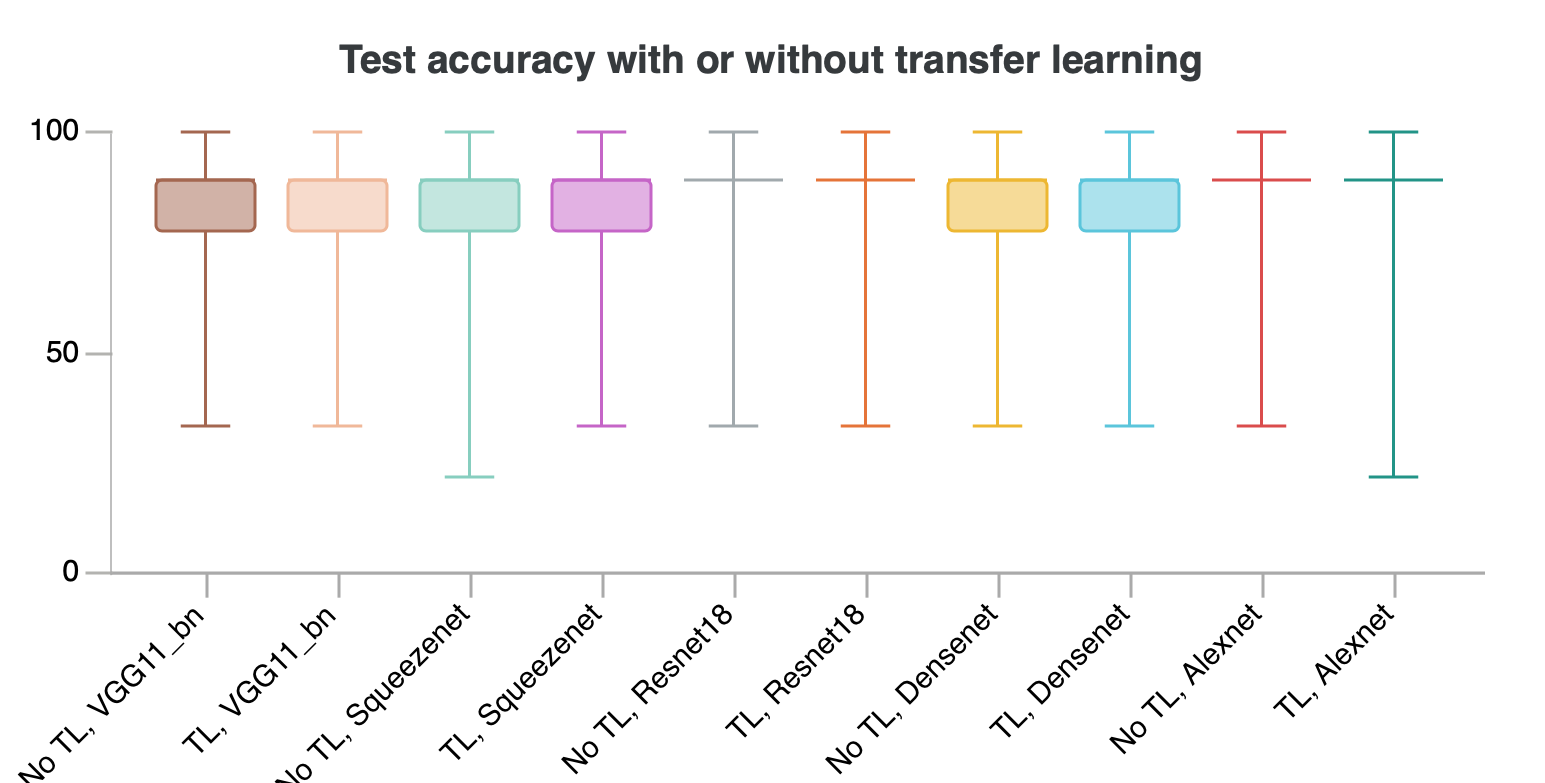
\includegraphics[width=\linewidth]{fig/results/wandb/second_handmade_sweep/charts/Section-13-Panel-1-nk6ghsz6f.png}
		\caption{Test accuracy}
		\label{fig:res:shm:tl:ta}
	\end{subfigure}
	\begin{subfigure}{0.49\textwidth}
		\centering
		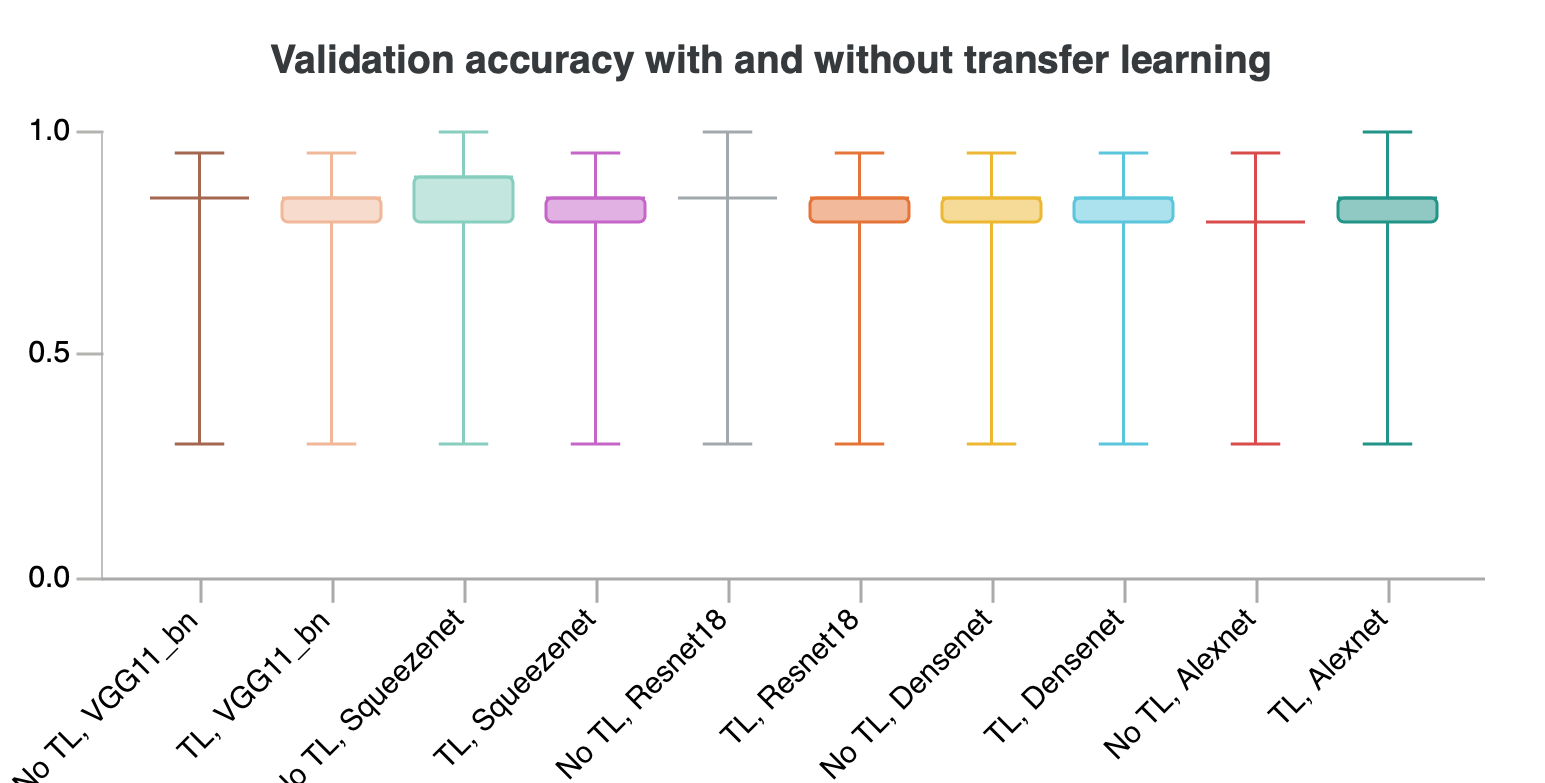
\includegraphics[width=\linewidth]{fig/results/wandb/second_handmade_sweep/charts/Section-13-Panel-0-hqve9y31m.png}
		\caption{Validation accuracy}
		\label{fig:res:shm:tl:va}
	\end{subfigure}
	\caption{Validation and test accuracy box plot for different model architectures with or without transfer learning (TL).}
	\label{fig:res:shm:tl}
\end{figure}

\subsection{Other parameter influences}
The settings for the 40 best runs are visualized in Figure \ref{fig:res:shm:params}. For every model architecture some different hyperparameters are listed with their values for different training runs. From left to right we see the model name, the amount of epochs for the training, the batch size, whether or not transfer learning is used and finally the learning rate. Since this graph shows the top 40 runs the amount of runs starting from a single model name defines its presence in this top 40. Squeezenet and Resnet18 are represented by a lot of runs where the most green lines start from Squeezenet. This green lines indicate a validation accuracy of more than 80\% for that run.

Other things we can learn from this graph are:
	\begin{itemize}
		\item  The epochs have a significant contribution to the validation accuracy where the amount of epochs can be finetuned between 30 epochs and 47 epochs for best results.
		\item A batch size between 10 and 4 seems good but doesn't contribute that much to the final results since the spread of runs across the different batch sizes is pretty even.
		\item There are more runs in the top 40 that doesn't use transfer learning. This means the transfer learning doesn't affect the results in a positive way for the most part.
		\item The learning rate used for adjusting the weights can differ highly from one run to the other. No points on the learning rate graph actually are significantly more populated than others. The learning rate can be set to higher and lower values for further testing.
	\end{itemize}


	\begin{figure}[hbtp]
		\centering
		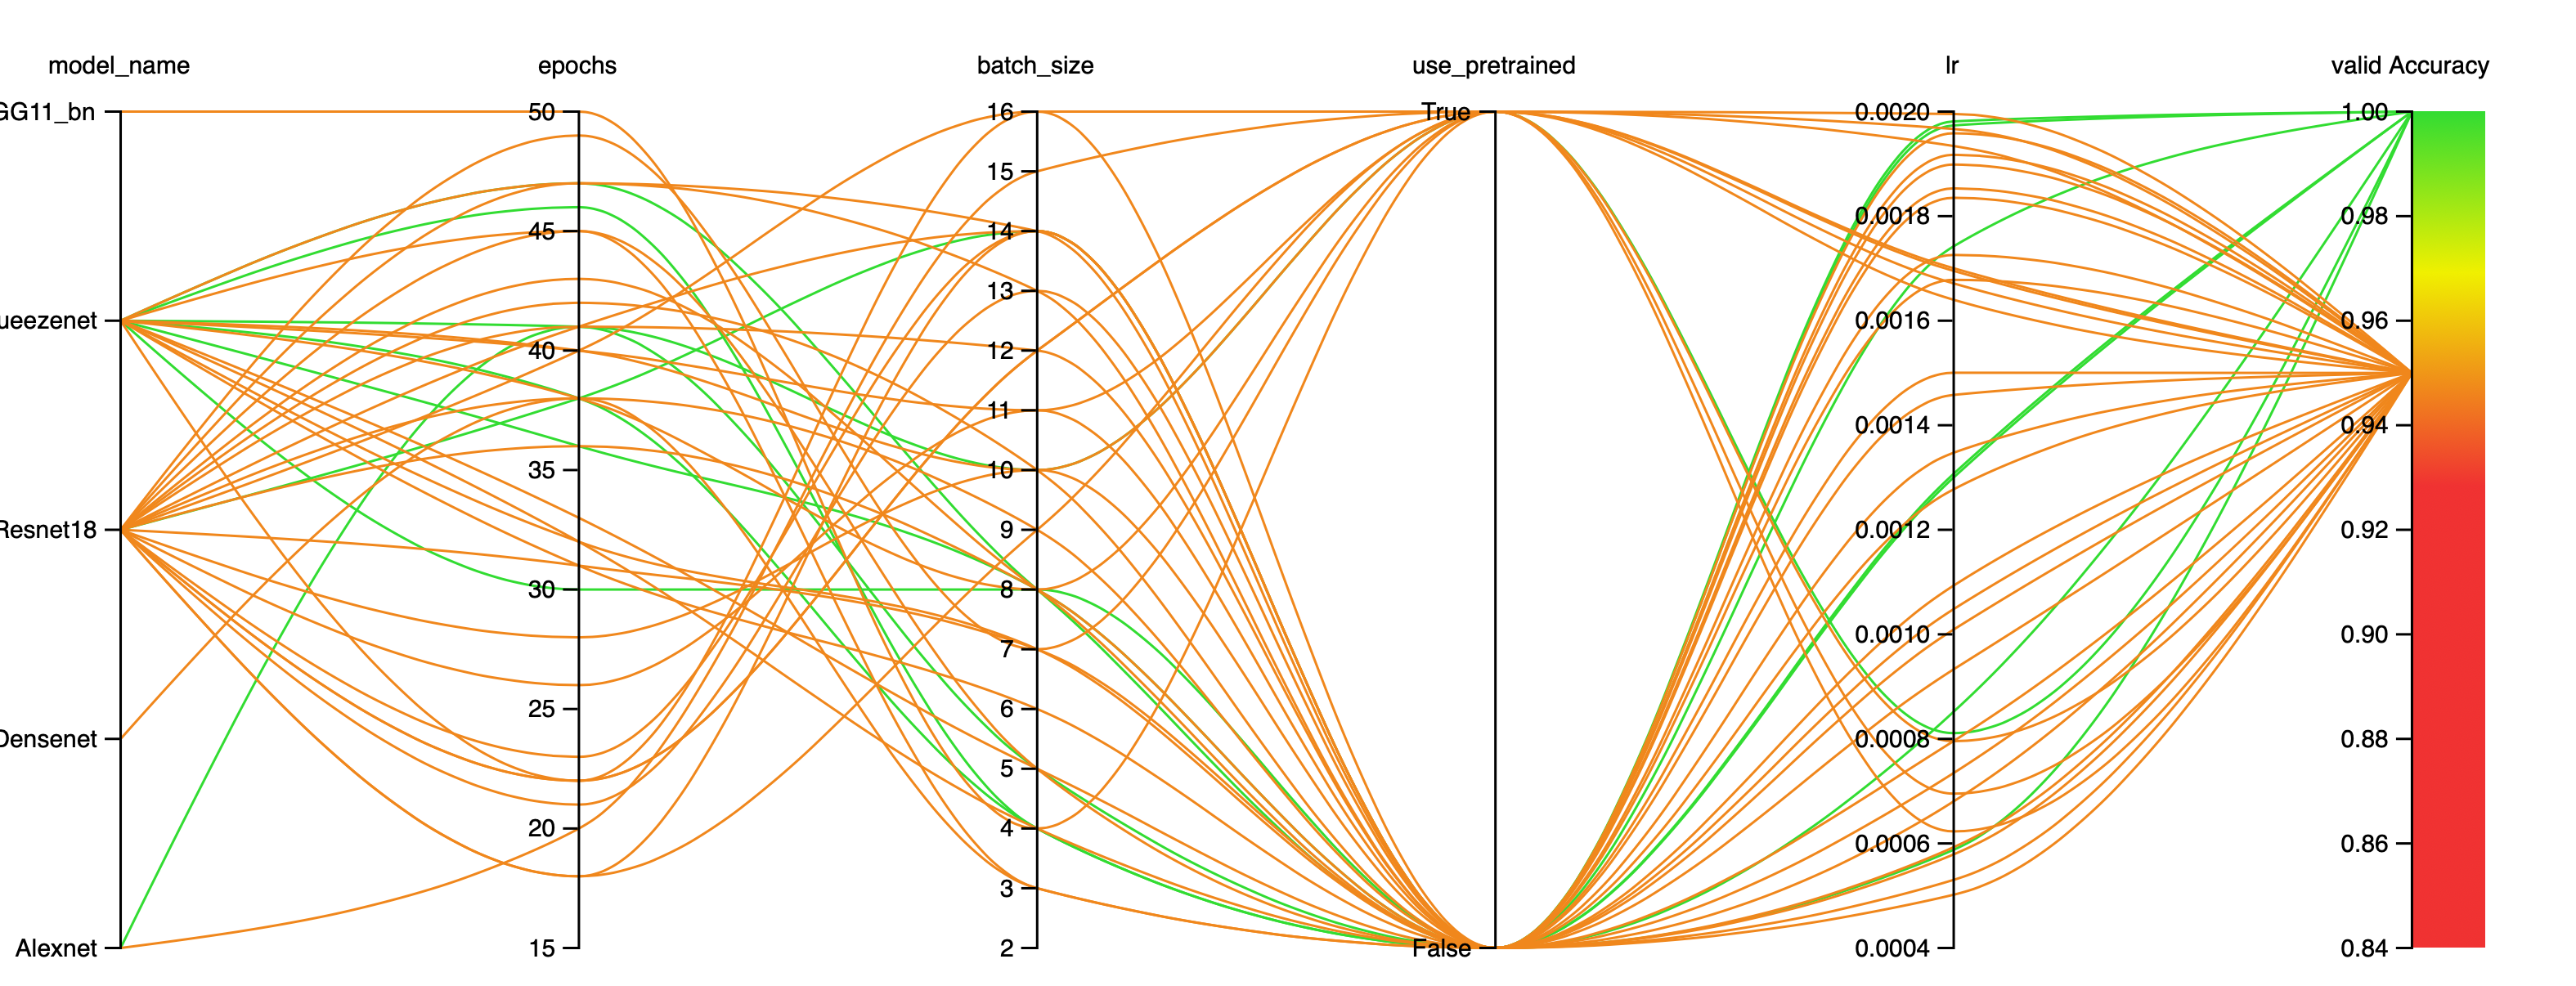
\includegraphics[width=\textwidth]{fig/results/wandb/second_handmade_sweep/charts/Section-21-Panel-0-xfrvxv29l.png}
		\caption{Parameter influence on validation accuracy.}
		\label{fig:res:shm:params}
	\end{figure}

\subsection{Test images}
Since the test accuracy was so high only a few images were falsely predicted thus it is not relevant to show images of these results.

\begin{comment}
\begin{figure}[hbtp]
	\begin{subfigure}{0.31\textwidth}
	\centering
	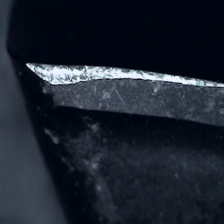
\includegraphics[width=\linewidth]{fig/results/wandb/second_handmade_sweep/images/pred0-truth0.png}
	\caption{Truth: High \\Predicted: High}
	\end{subfigure}
	\hspace*{\fill}
	\begin{subfigure}{0.31\textwidth}
	\centering
	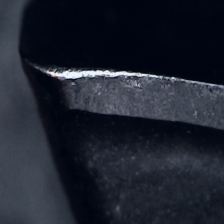
\includegraphics[width=\linewidth]{fig/results/wandb/second_handmade_sweep/images/pred2-truth2.png}
	\caption{Truth: Medium \\Predicted: Medium}
	\end{subfigure}
	\hspace*{\fill}
	\begin{subfigure}{0.31\textwidth}
	\centering
	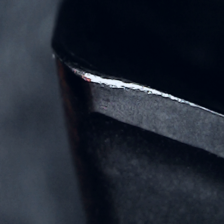
\includegraphics[width=\linewidth]{fig/results/wandb/second_handmade_sweep/images/pred1-truth1.png}
	\caption{Truth: Low \\Predicted: Low}
	\end{subfigure}
	\caption{Result images with their results.}
\end{figure}
\end{comment}

\section{Birthday dataset results}
	For the birthday dataset there are no results available because the dataset was not considered good which was discussed in \ref{sec:impl:dataset:birthday}.

\section{Spaghetti dataset results}
	The spaghetti dataset was the first dataset to capture all of the currently available tool inserts. The different insert types are all in this one dataset where white as well as red lighting was used. 158 runs where completed with different parameters to generate the following results.
	For this third dataset the overall results are discussed in the first section where we take a look at the five best runs. After the general results we dive deeper into the different model architectures. After which some differences will be discussed.

	\subsection{Overall results for five best runs}
		The five best results are discussed to get a quick overview of the performance of this dataset on the chosen model architectures. The test accuracy for the five best runs is shown in Figure \ref{fig:res:sd:ta}. The maximum test accuracy is 82.1\%. To dive deeper in the training we take a look at the training accuracy in Figure \ref{fig:res:sd:tra} the training accuracy is very high near 100\%. The high training accuracy means the training pictures get predicted correctly but the other general pictures get predicted wrong for almost 20\% of the pictures. To take a deeper look into this difference between testing and training accuracy we take a look at the validation accuracy during training. If the training accuracy would increment and the validation accuracy would decrement after a time the model might be overfitting. Figure \ref{fig:res:sd:va} shows the training and validation accuracy during training. There is no overfitting seen on this graph so the model just isn't powerful enough for the task or the dataset is too small.
	\begin{figure}[hbtp]
		\begin{subfigure}{0.49\textwidth}
			\centering
			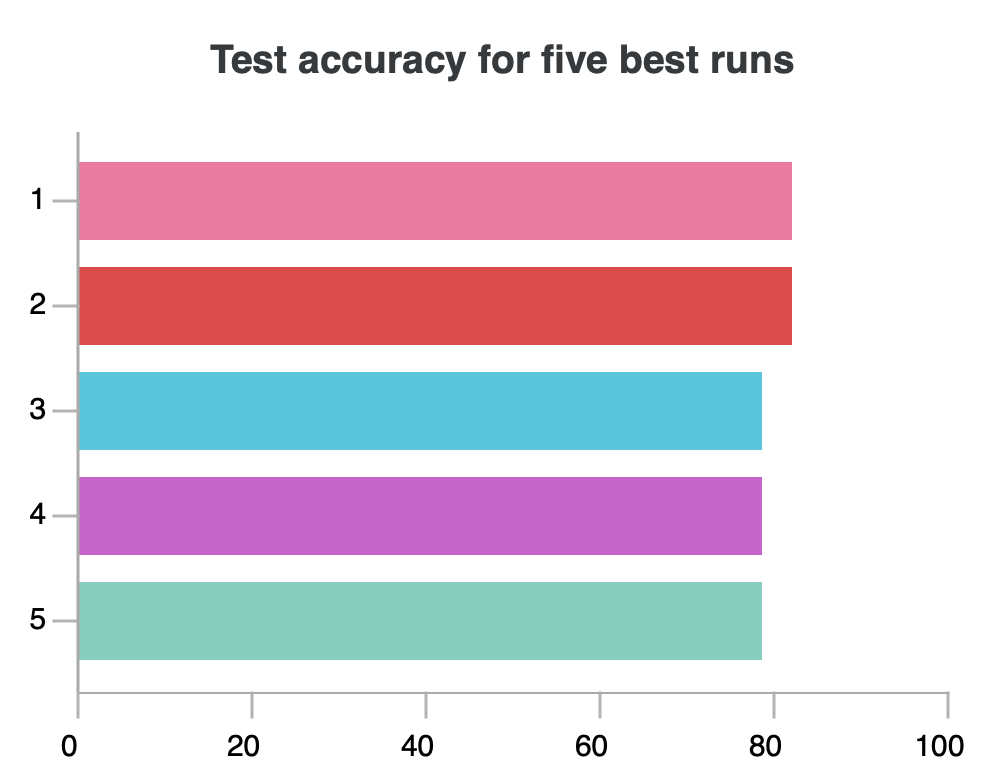
\includegraphics[width=\linewidth]{fig/results/wandb/spaghetti_dataset/charts/Section-2-Panel-2-od5lt0wga}
			\caption{Test accuracy}
			\label{fig:res:sd:ta}
		\end{subfigure}
		\hspace*{\fill}
		\begin{subfigure}{0.49\textwidth}
			\centering
			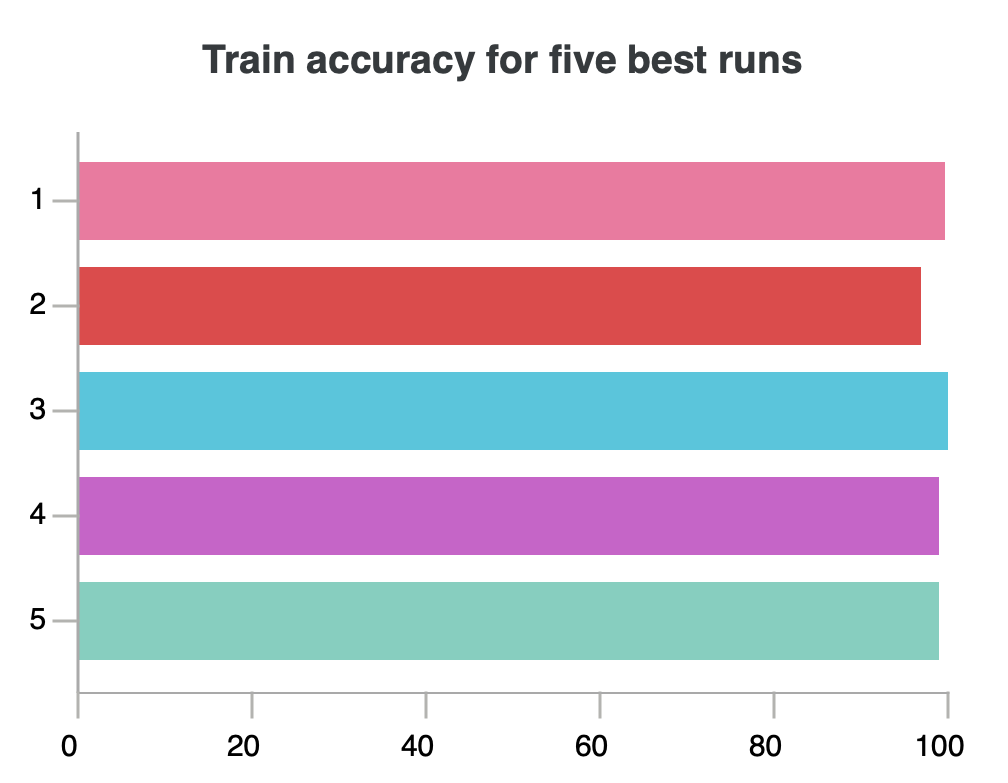
\includegraphics[width=\linewidth]{fig/results/wandb/spaghetti_dataset/charts/Section-2-Panel-1-vxyqvv7et}
			\caption{Train accuracy}
			\label{fig:res:sd:tra}
		\end{subfigure}
		\hspace*{\fill}
		\centering
		\begin{subfigure}{0.6\textwidth}
			\centering
			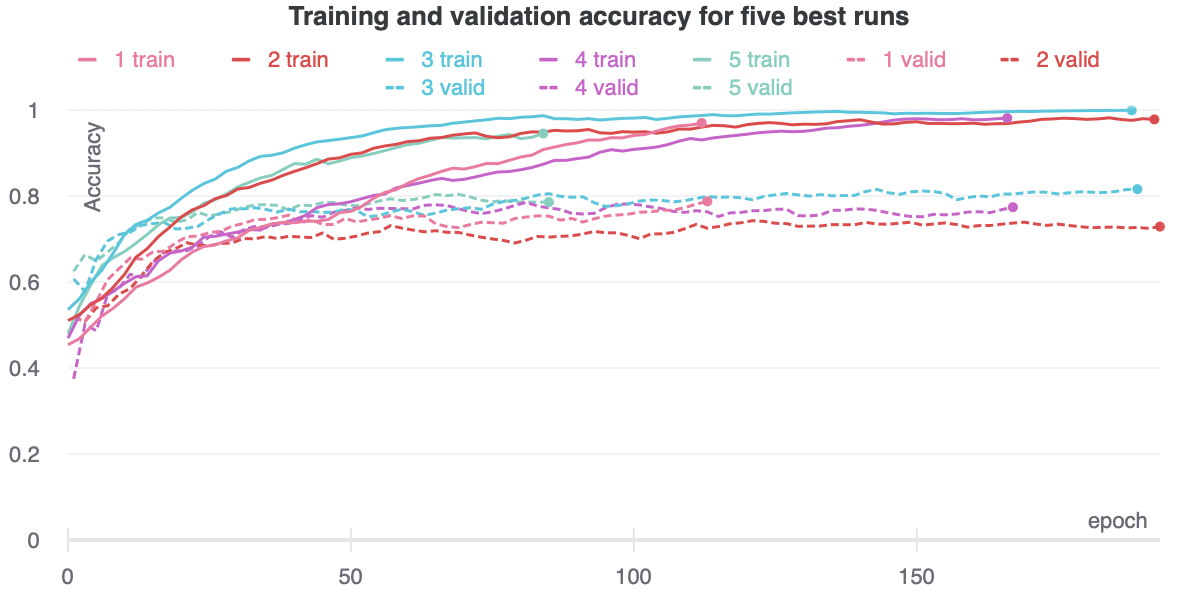
\includegraphics[width=\linewidth]{fig/results/wandb/spaghetti_dataset/charts/train_valid_accuracy.png}
			\caption{Training and validation accuracy}
			\label{fig:res:sd:va}
		\end{subfigure}
		\hspace*{\fill}
		\caption{Test, train and validation accuracy for the five best runs based on their test accuracy scores.}
	\end{figure}
	
	\subsection{Comparison between different model architectures}
		Just like we did for the Second handmade dataset, the results for different model architectures are compared. The test accuracy, validation accuracy and influence of transfer learning are analysed.
		\subsubsection{Test accuracy}
			On the first graph the test best test accuracy for every model is plotted. Densenet achieved the best accuracy for predicting the wear class of images on the test set. 78\% of images were correctly predicted. The other architectures aren't far behind on the accuracy with 75\%. Resnet 18 on the other hand is performing worse with a test accuracy of only 67\%. On this first opinion Densenet seems to be the best model for this classification task.

	\begin{figure}[hbtp]
		\centering
		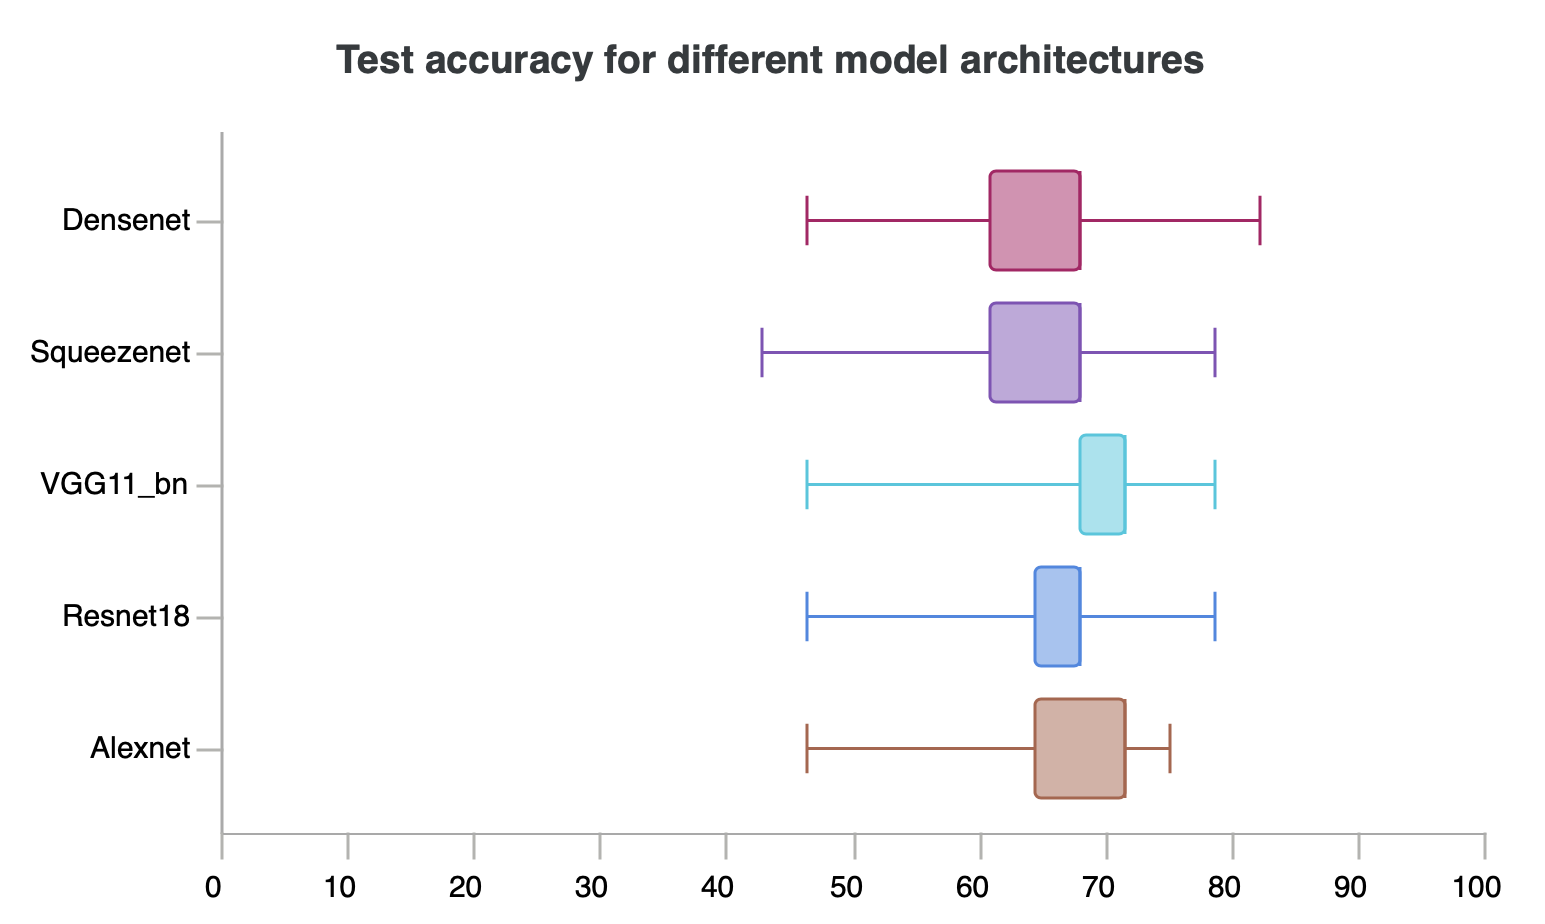
\includegraphics[width=0.5\linewidth]{fig/results/wandb/spaghetti_dataset/charts/Section-6-Panel-0-5bt9qjs32}
		\caption{Test accuracy}
	\end{figure}
	
		\subsection{Validation Accuracy}
To further check the performance of the models a graph is shown in figure below. Here the validation accuracy is plotted for every model with its minima and maxima in shadow. There is not much of an inclining curve to this graph where normally the graph would go up in the first half and stabilise at the end.

Squeezenet and VGG11\_bn  seem to have trained to the highest validation accuracy of 82\%. This is an indication on how well the model will react on new images like the images from the test set. Densenet has an accuracy of 78\%, Alexnet an accuracy of 75\% and finally Resnet 18 with an accuracy of 73\%. There must be noticed that Resnet 18 only got tested in 3 different parameter configurations whereas the others where optimized a bit more.
	
	
	Table \ref{tab:results:spaghetti:valacc} shows the results for the different model architectures where the test and validation accuracy predict almost the same order for best model architecture. VGG11\_bn and Densenet take the lead here. These networks are complexer with more layers and more parameters. The validation accuracy during training is also plotted for the best runs of each architecture. This can be seen in Figure \ref{fig:results:spaghetti:architectures:valacc}
	\begin{table}[h!]
			\begin{tabular}{ c | c c }
			%\caption{Confusion matrix for tests of Second handmade dataset}
			Model name		& Validation Accuracy 	& Validation accuracy sorted on test accuracy	\\ \hline
			VGG11\_bn 			& 84\%						& 82\%					\\
		 	Densenet 				& 84\%						& 82\% 				\\ 
		 	Alexnet			& 82\%							& 82\%					\\
		 	Squeezenet			& 82\%							& 78\%					\\
		 	Resnet 18 		& 80\%						& 80\%					\\
			\end{tabular}
			\caption{Validation accuracy plotted for best model per architecture. In first column sorted on best validation accuracy, in second column sorted on best test accuracy.}
			\label{tab:results:spaghetti:valacc}
		\end{table}
		
	\begin{figure}[hbtp]
	\centering
	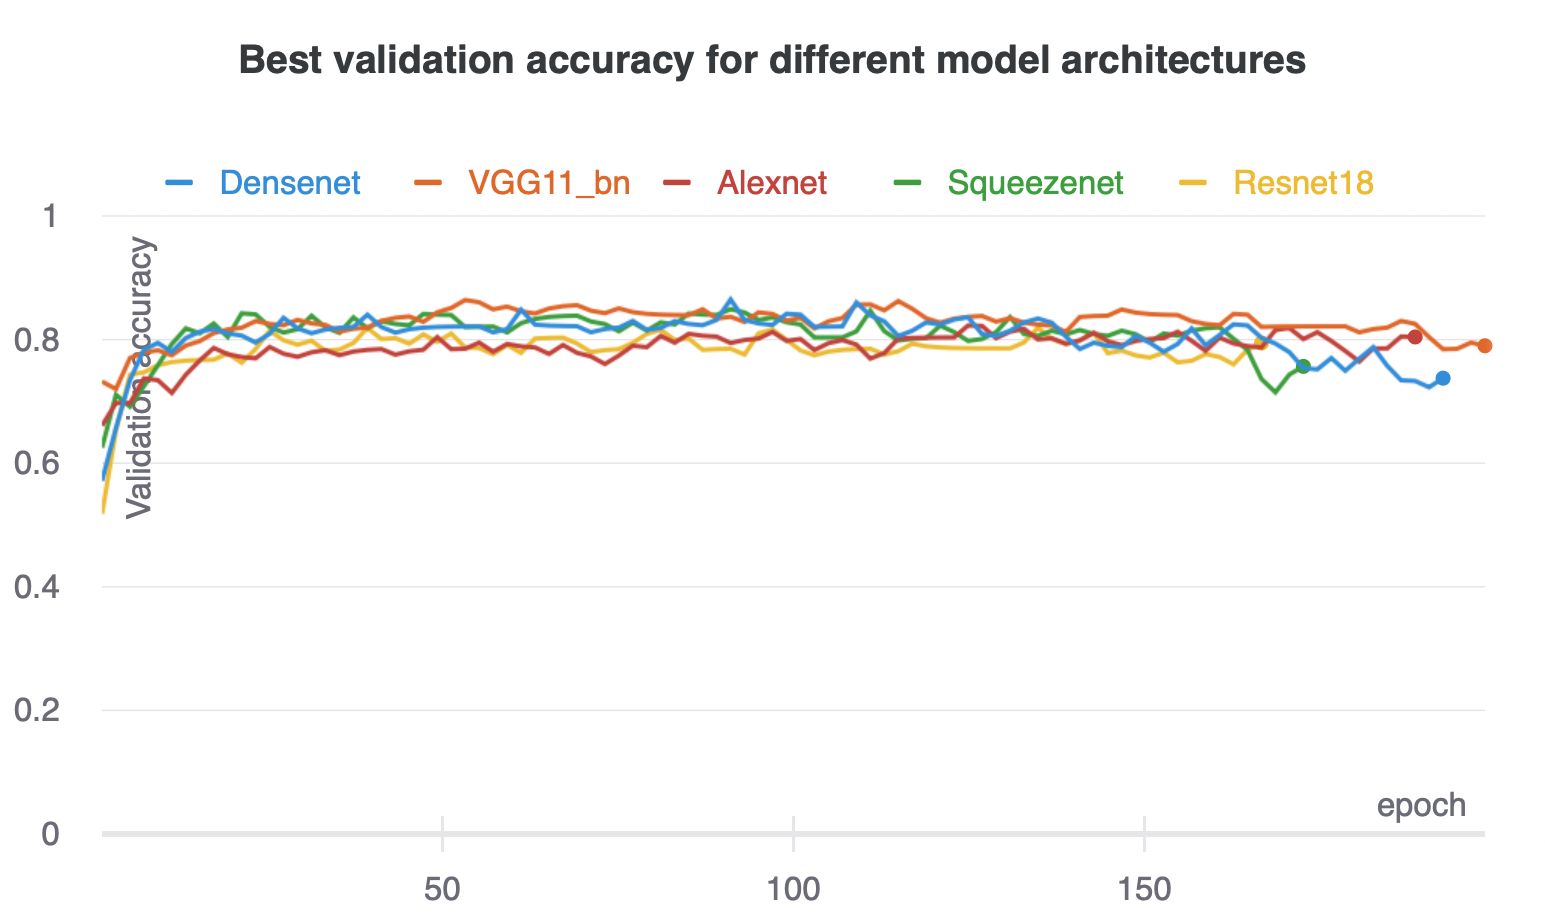
\includegraphics[width=0.6\linewidth]{fig/results/wandb/spaghetti_dataset/charts/Section-13-Panel-0-yf0a5rsos}
	\caption{Best validation accuracy for different model architectures plotted in relation to the amount of epochs.}
	\label{fig:results:spaghetti:architectures:valacc}
	\end{figure}

	\subsection{Influence of transfer learning on the results}
		The transfer learning influence is plotted in Figure \ref{fig:res:sd:ta:tl} for the test and validation accuracy. Transfer learning generally seems to have an effect on this dataset where the runs with transfer learning score on average 2\% better and the maximum result is 5\% better which is a significant improvement over the runs without transfer learning. 
		
		The same difference is also compared for all different model architectures in Figure \ref{fig:res:sd:ta:tl:arch} where the test accuracy is laid out. Squeezenet, Resnet 18, Densenet and Alexnet all benfit from transfer learning. VGG11\_bn on the other hand doesn't benefit from transfer learning and produces the same results for both settings.
		
		As there are significant differences in the results for training with or without transfer learning the training of the models is examined. First the median and standard deviation of the validation accuracy during training is plotted in Figure \ref{fig:res:sd:va:tl}, secondly the train accuracy is plotted in Figure \ref{fig:res:sd:tra:tl}. 
		When looking at the validation accuracy, the learning curve with transfer learning inclines a bit before the curve without transfer learning. Using a pre-trained network speeds up the initialisation of the network but also uses more epochs to finish the training. There are no differences worth noting in the course of the training accuracy.

	\begin{figure}[hbtp]
		
		\begin{subfigure}{0.49\textwidth}
		\centering
		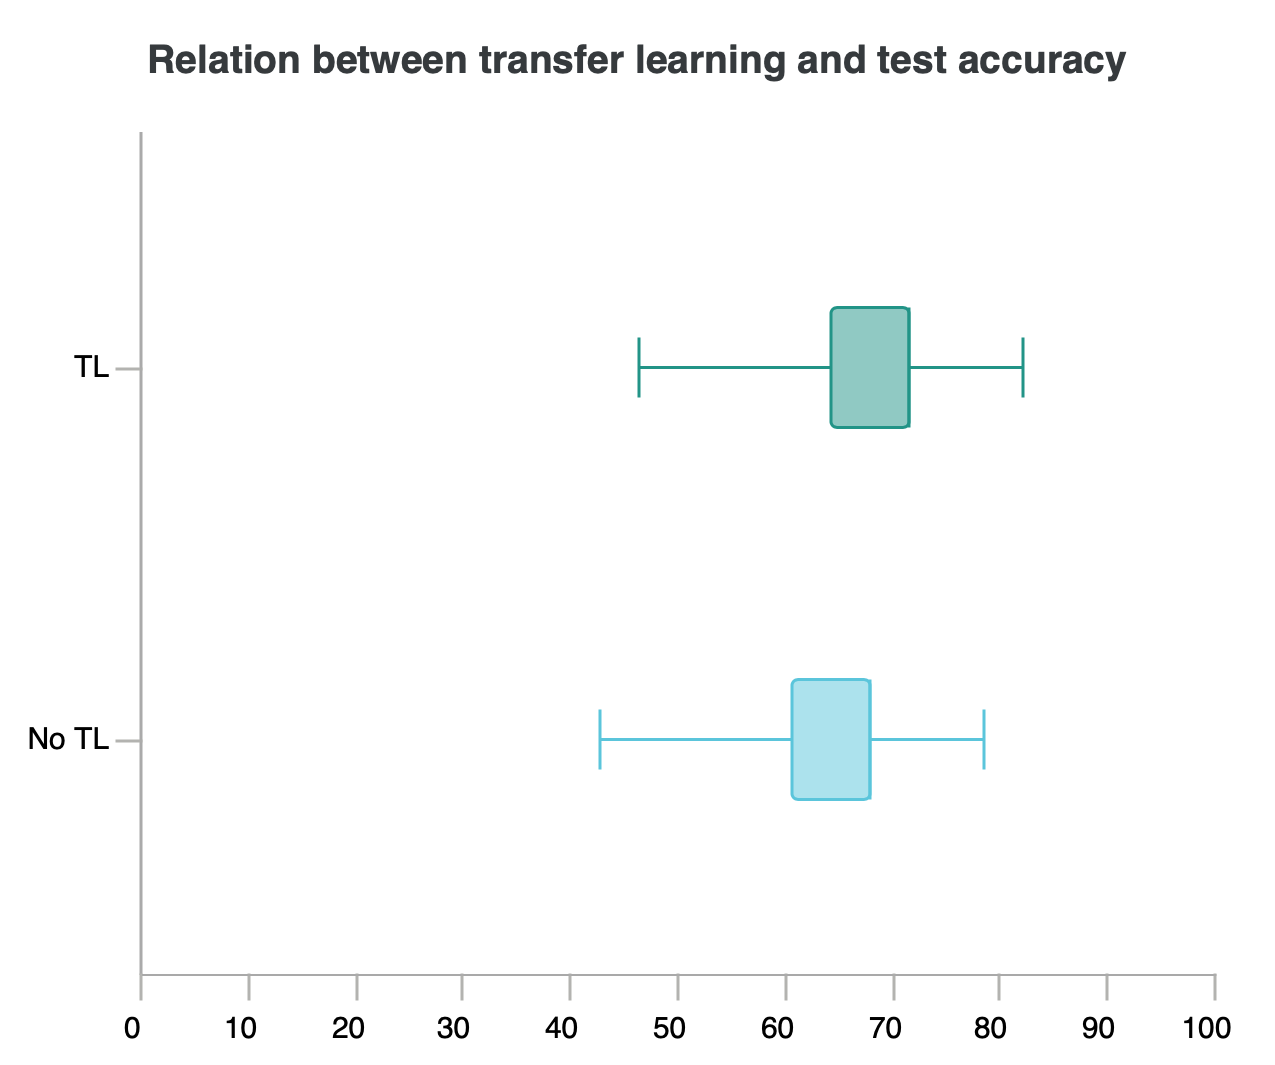
\includegraphics[width=\linewidth]{fig/results/wandb/spaghetti_dataset/charts/Section-8-Panel-0-tz8zymurl}
		\caption{Test accuracy for all runs with and without transfer learning.}
		\label{fig:res:sd:ta:tl}
		\end{subfigure}
		\hspace*{\fill}
		\begin{subfigure}{0.49\textwidth}
		\centering
		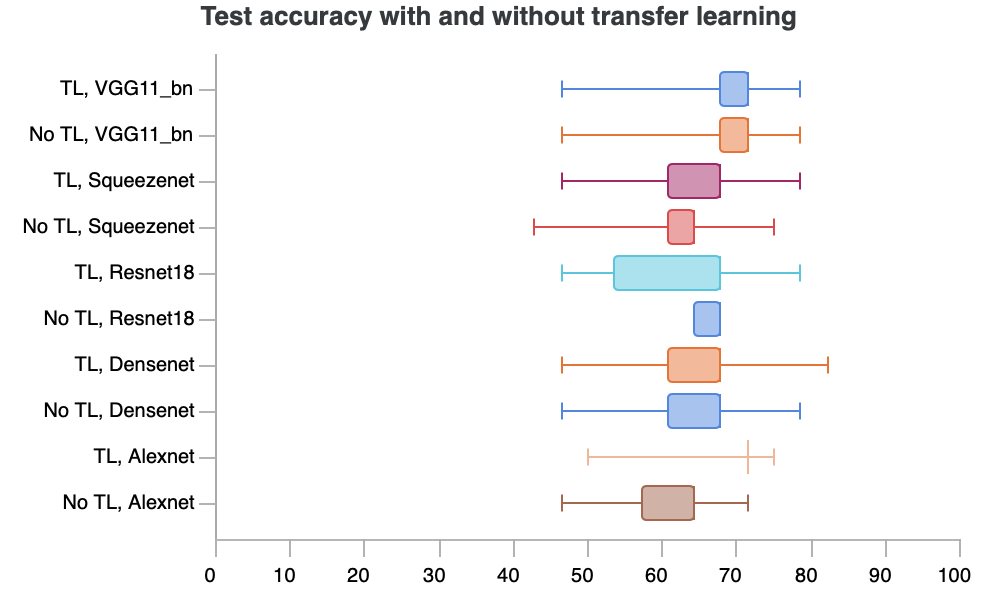
\includegraphics[width=\linewidth]{fig/results/wandb/spaghetti_dataset/charts/test_accuracy_architectures.png}
		\caption{Test accuracy with or without transfer learning for different model architectures. }
		\label{fig:res:sd:ta:tl:arch}
		\end{subfigure}
		\hspace*{\fill}
		\begin{subfigure}{0.49\textwidth}
		\centering
		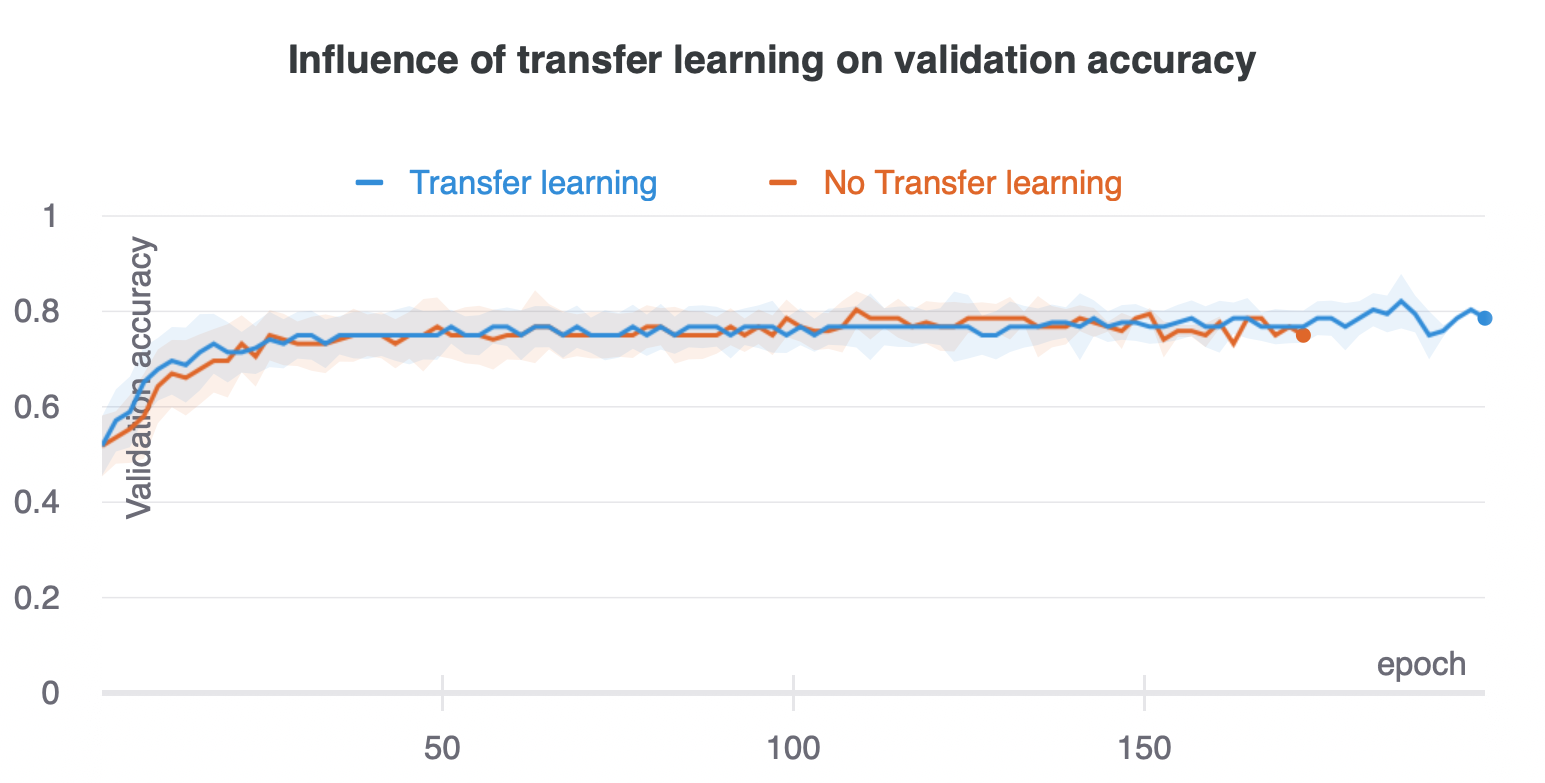
\includegraphics[width=\linewidth]{fig/results/wandb/spaghetti_dataset/charts/Section-10-Panel-0-rj7vtzd5m}
		\caption{Validation accuracy }
		\label{fig:res:sd:va:tl}
		\end{subfigure}
		\hspace*{\fill}
		\begin{subfigure}{0.49\textwidth}
		\centering
		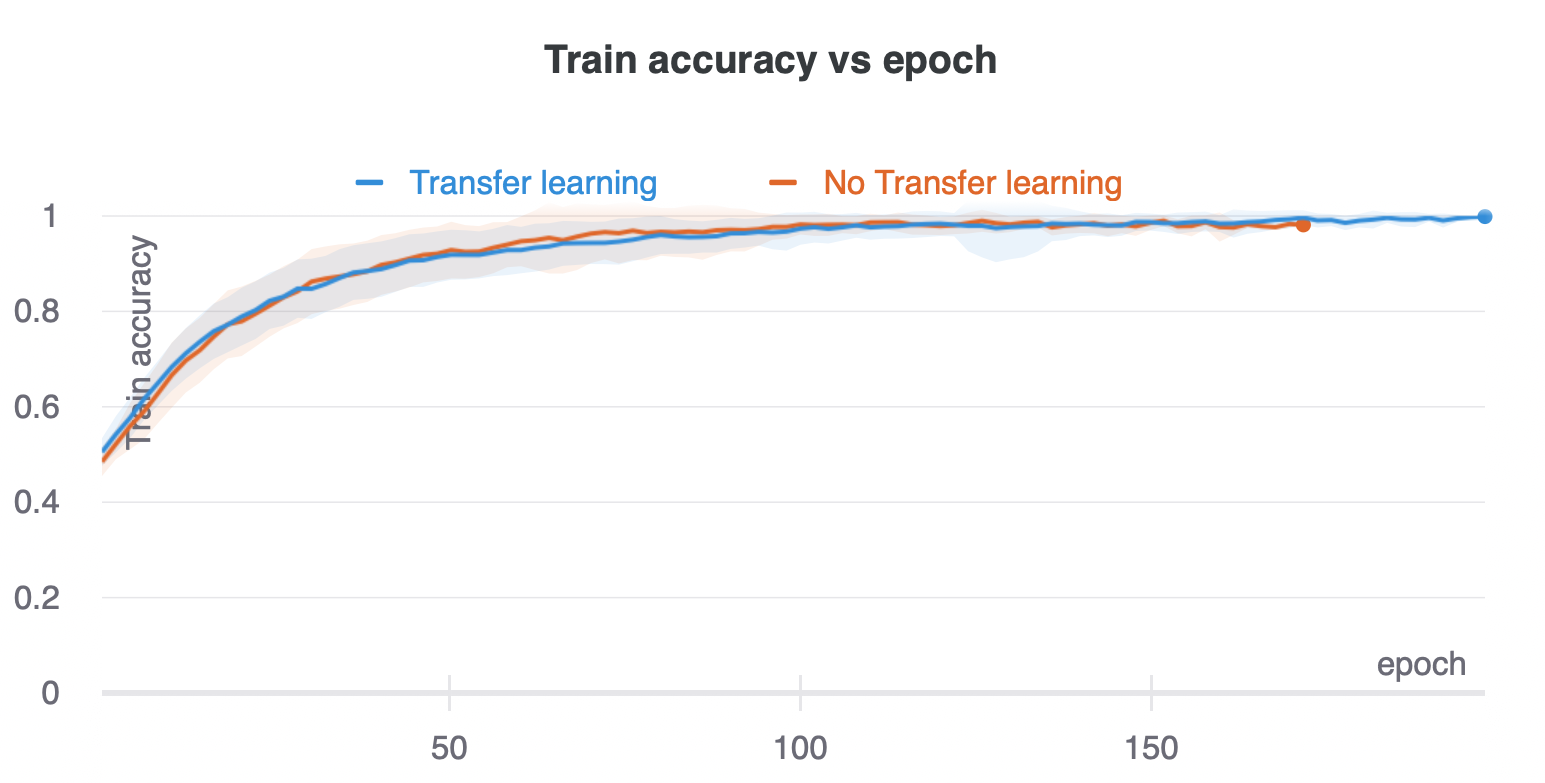
\includegraphics[width=\linewidth]{fig/results/wandb/spaghetti_dataset/charts/Section-10-Panel-1-gr2eg8ssf}
		\caption{Training accuracy}
		\label{fig:res:sd:tra:tl}
		\end{subfigure}
		\caption{Test accuracy for models trained with and without transfer learning. In picture a) a general overview of all performed tests. in picture b) a comparison between different model architectures. Picture c and d provide the differences during training for validation accuracy and training accuracy respectively.}
	\end{figure}
		



\subsection{Red vs White}
\label{sec:results:spaghetti:colour}
	 For further investigation of the lighting color effects on the results, the median and standard deviation of the test and validation accuracy are plotted in Figure \ref{ref:res:sd:ta:rw} and \ref{fig:res:sd:va:rw}. For the validation accuracy there is a small difference of 4\% between the two curves where the white lighting seems to perform better. A similar result can be seen for the median of the test accuracy however the best results got achieved by the dataset with red lighting. 

	\begin{figure}[hbtp]
		\begin{subfigure}{0.49\textwidth}
		\centering
		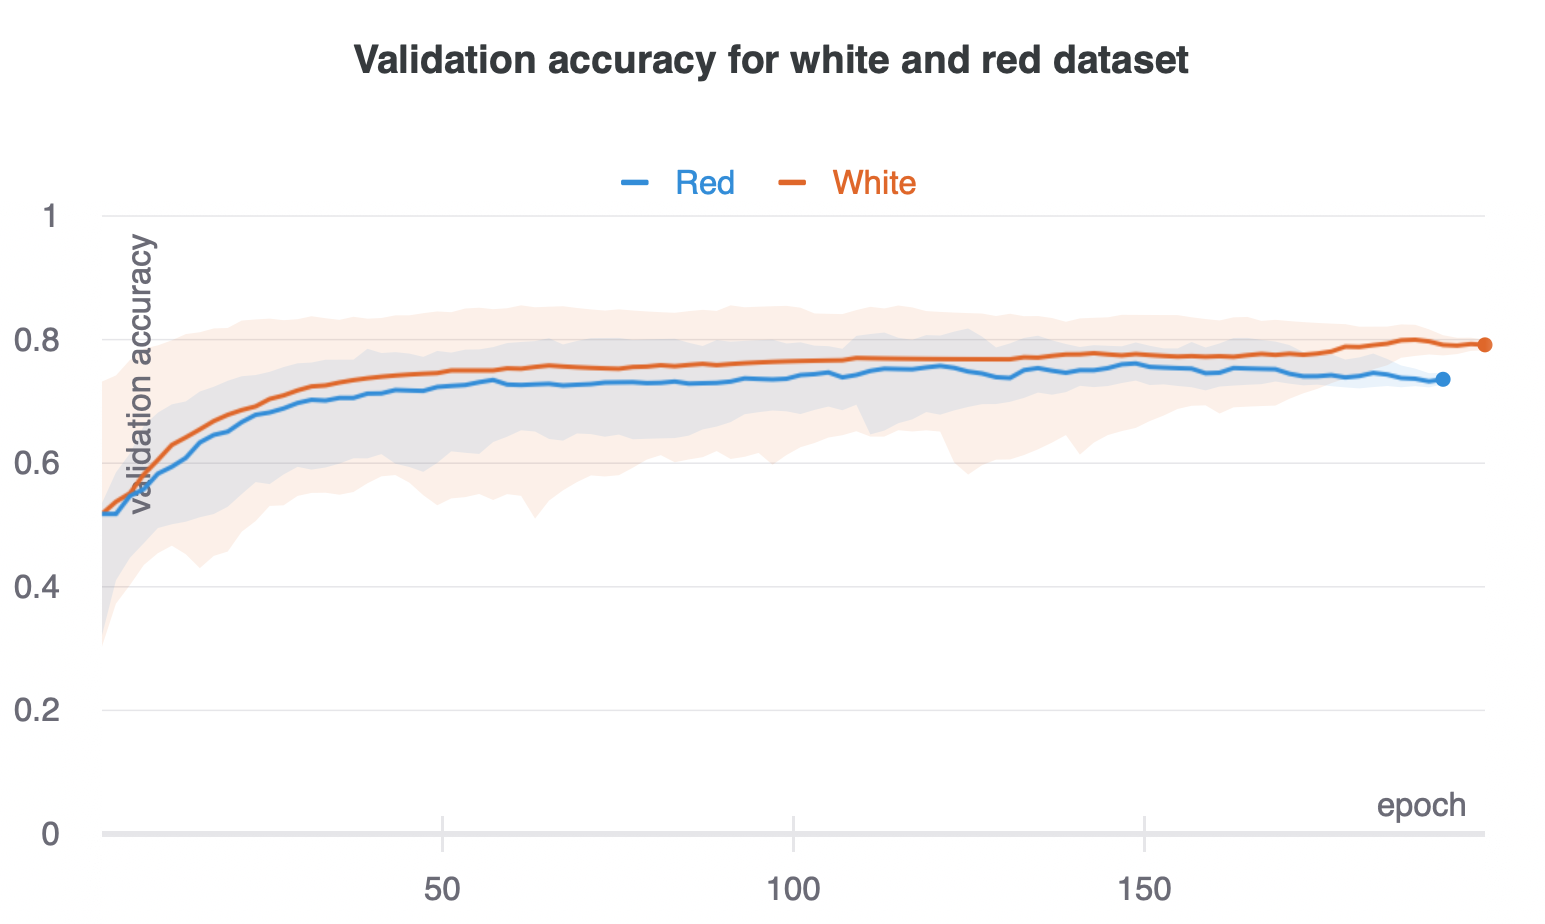
\includegraphics[width=\linewidth]{fig/results/wandb/spaghetti_dataset/charts/Section-16-Panel-0-gkiaebqxq}
		\caption{Test accuracy.}
		\label{ref:res:sd:ta:rw}
		\end{subfigure}
		\hspace*{\fill}
		\begin{subfigure}{0.49\textwidth}
		\centering
		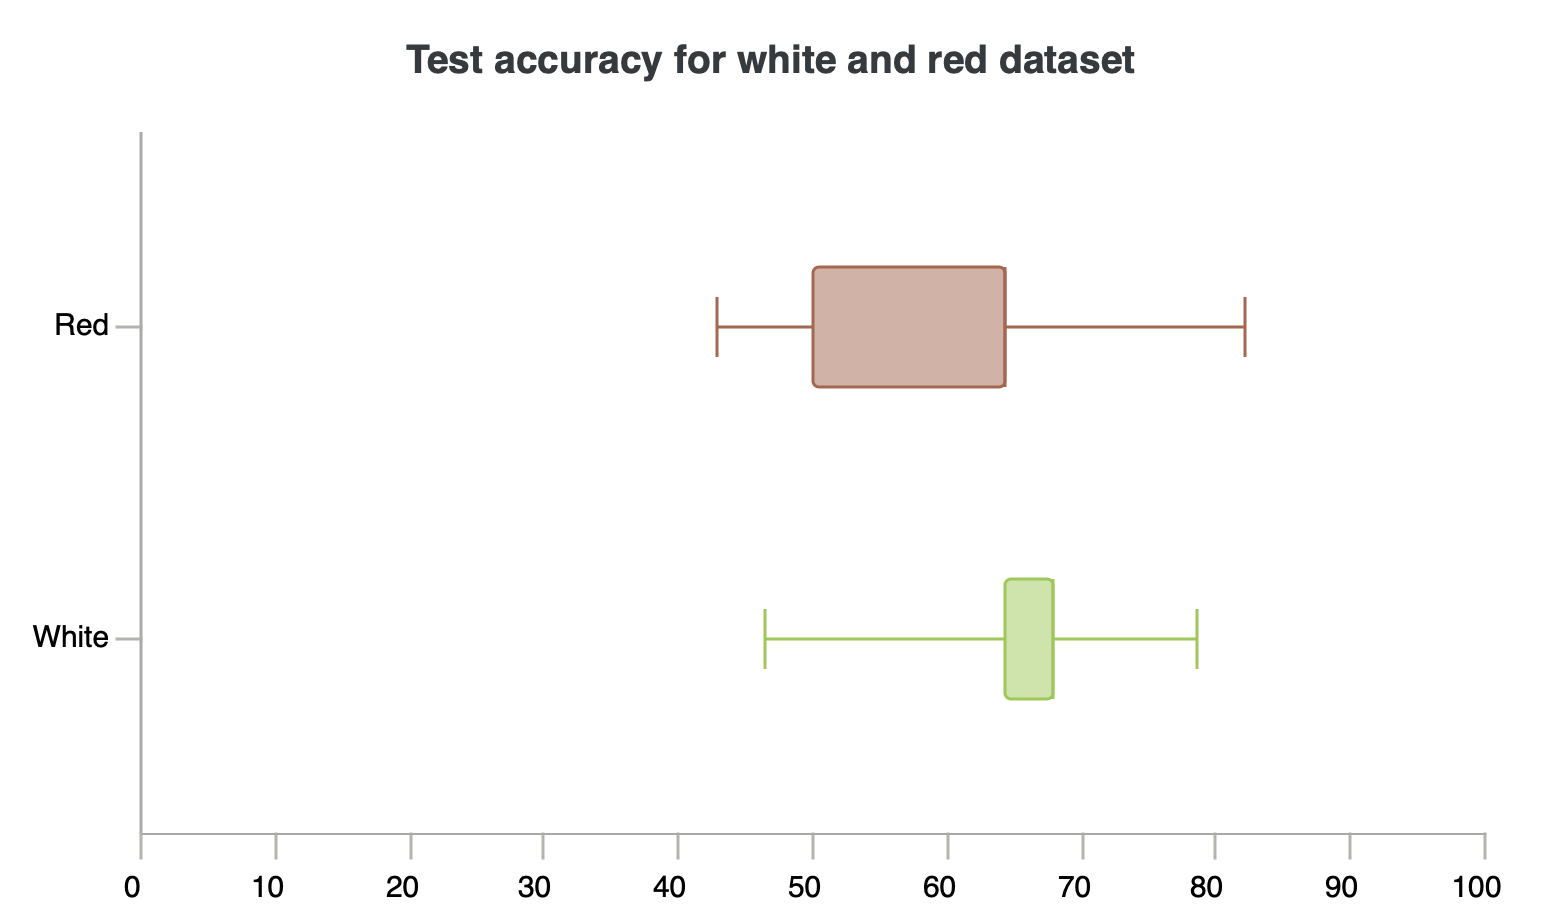
\includegraphics[width=\linewidth]{fig/results/wandb/spaghetti_dataset/charts/Section-16-Panel-1-lgbosq568}
		\caption{Validation accuracy}
		\label{fig:res:sd:va:rw}
		\end{subfigure}
		\caption{Test and validation accuracy for a different led color.}
	\end{figure}
	

\subsection{Training runs}
	On figure \ref{fig:res:sd:tr} different runs with different parameters are displayed. Here can be seen that more green lines start from the white dataset. This corresponds to earlier findings where was stated that the white dataset performed better on average. The batch size can be finetuned between 16 and 2. The amount of epochs can be increased in an attempt to improve the results, however on Figure \ref{fig:res:sd:va} the validation accuracy seems to be stable at the end where adding more epochs wouldn't change much on the results. The learning rate can be kept between 0 and 0.002. Using transfer learning isn't a deciding factor for good results. 

	\begin{figure}[hbtp]
		\centering
		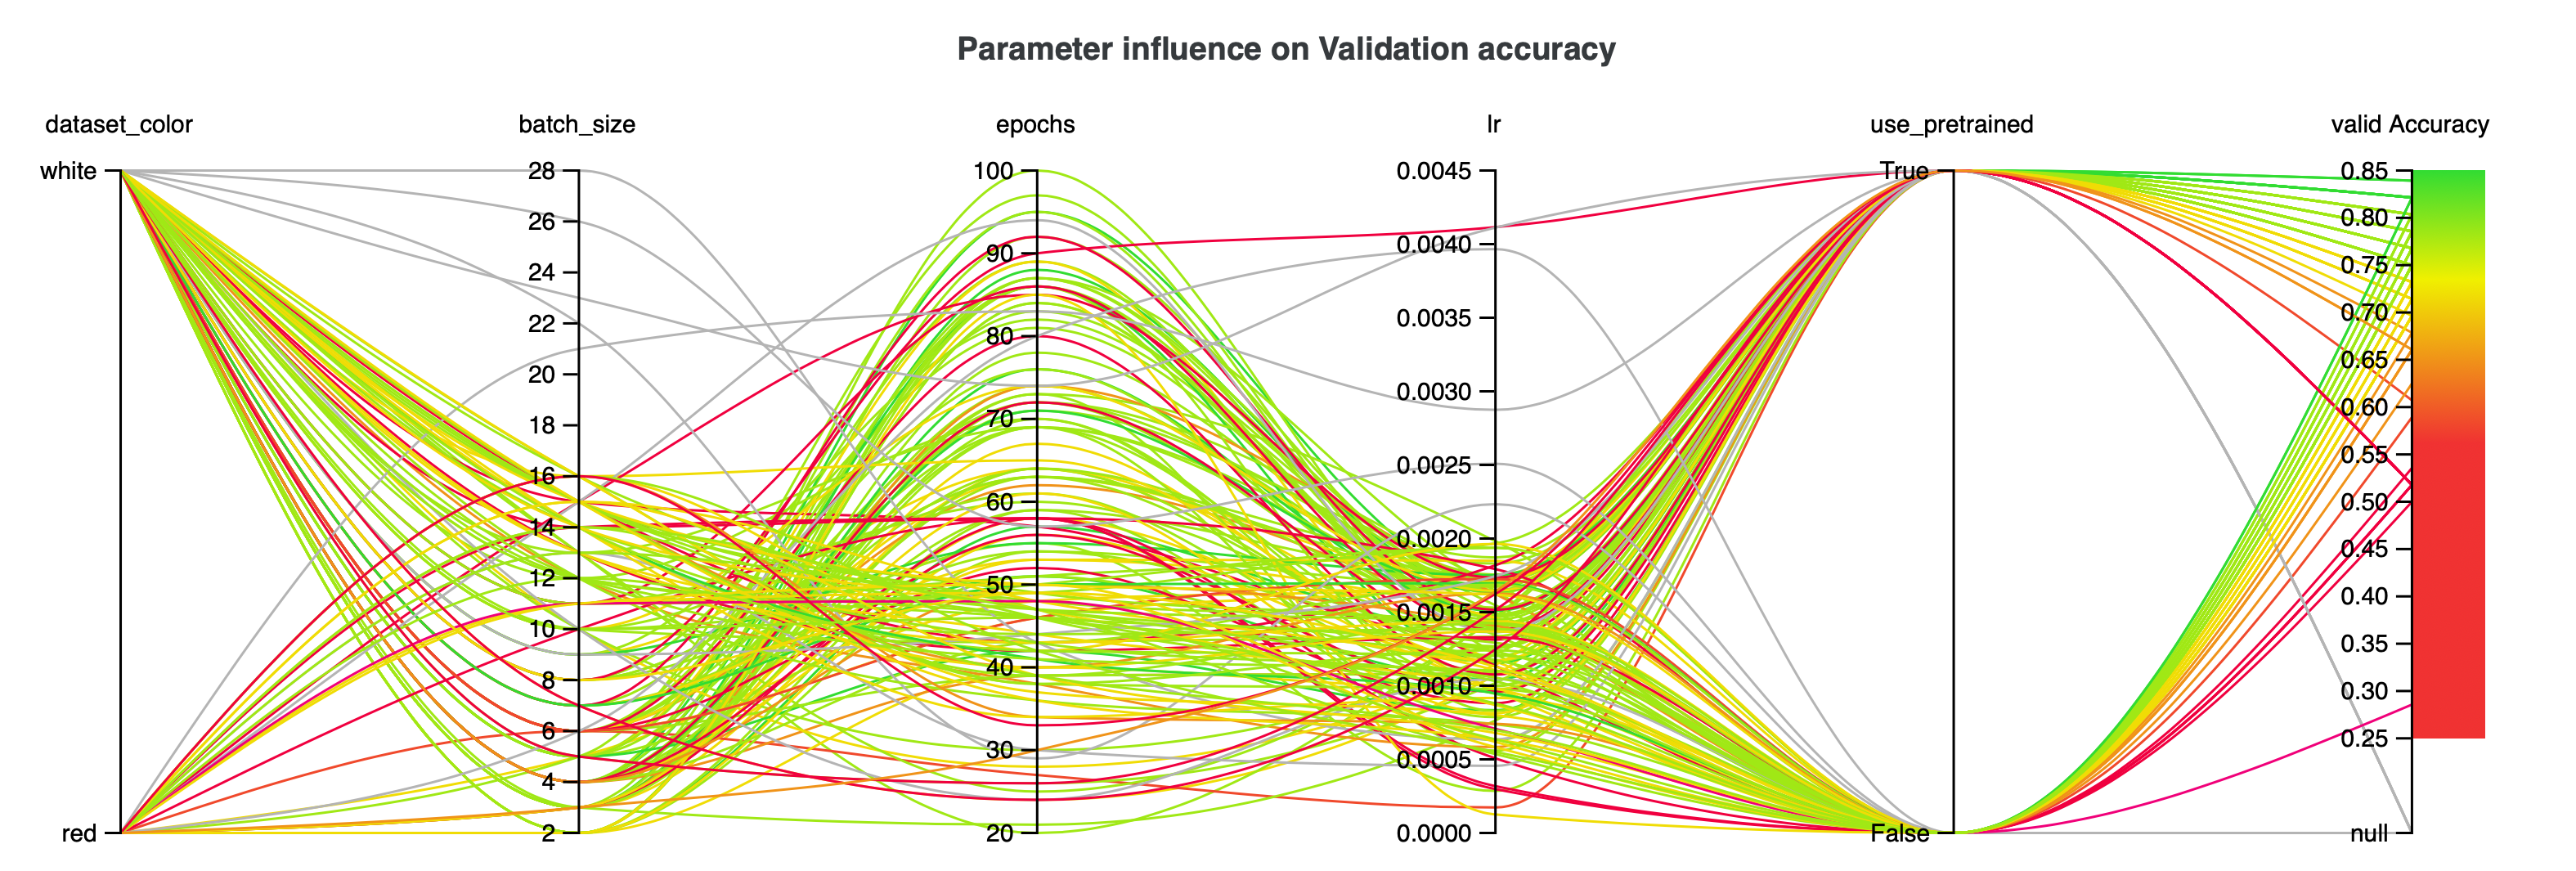
\includegraphics[width=\linewidth]{fig/results/wandb/spaghetti_dataset/charts/Section-19-Panel-0-alqny4fc9}
		\caption{Parameter influence on validation accuracy.}	
		\label{fig:res:sd:tr}
	\end{figure}
	
\subsection{Test images}
	To illustrate the results, some test images from the white lighted part of the dataset are listed in Figure \ref{fig:res:sd:testimg}. One error is given in Figure \ref{fig:res:sd:testimg:error} where high wear was predicted for a medium wear insert. No hard mistakes where found in the outcome of this test.

	\begin{figure}[hbtp]
		\begin{subfigure}{.24\textwidth}
			\centering
			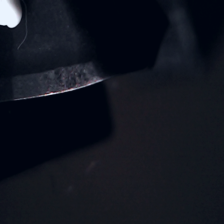
\includegraphics[width=\linewidth]{fig/results/wandb/spaghetti_dataset/images/media_images_Examples_142_p1_t1.png}
			\caption{Truth: Low \\Predicted: Low}
		\end{subfigure}
		\hspace*{\fill}
		\begin{subfigure}{.24\textwidth}
			\centering
			
\includegraphics[width=\linewidth]{fig/results/wandb/spaghetti_dataset/images/media_images_Examples_176_p2_t2.png}
			\caption{Truth: Medium \\Predicted: Medium}
		\end{subfigure}
		\hspace*{\fill}
		\begin{subfigure}{.24\textwidth}
			\centering
			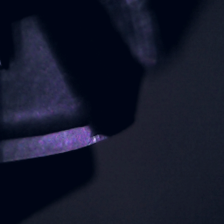
\includegraphics[width=\linewidth]{fig/results/wandb/spaghetti_dataset/images/media_images_Examples_144_p0_t2.png}
			\caption{Truth: Medium \\Predicted: High}
			\label{fig:res:sd:testimg:error}
		\end{subfigure}
		\hspace*{\fill}
		\begin{subfigure}{.24\textwidth}
			\centering
			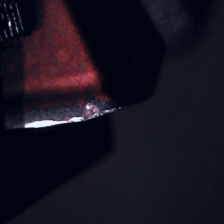
\includegraphics[width=\linewidth]{fig/results/wandb/spaghetti_dataset/images/media_images_Examples_102_p0_t0.png}
			\caption{Truth: High \\Predicted: High}
		\end{subfigure}
		\caption{Images with predictions from the spaghetti dataset with white lighting.}
		\label{fig:res:sd:testimg}
	\end{figure}

In Figure \ref{fig:res:sd:testimg:red} some outputs for the red dataset are listed. Figure \ref{fig:res:sd:testimg:red:error} displays an error where a medium wear inset was predicted as high wear. On this same picture is a big plastic piece visible in the picture. This possibly affects the result.
	\begin{figure}[hbtp]
		\begin{subfigure}{.24\textwidth}
			\centering
			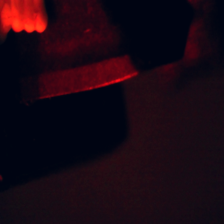
\includegraphics[width=\linewidth]{fig/results/wandb/spaghetti_dataset/images/media_images_Examples_r_194_p1_t1.png}
			\caption{Truth: Low \\Predicted: Low}
		\end{subfigure}
		\hspace*{\fill}
		\begin{subfigure}{.24\textwidth}
			\centering
			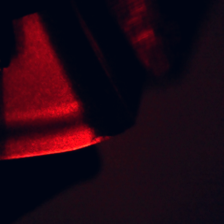
\includegraphics[width=\linewidth]{fig/results/wandb/spaghetti_dataset/images/media_images_Examples_r_172_p2_t2.png}
			\caption{Truth: Low\\Predicted: Low}
		\end{subfigure}
		\hspace*{\fill}
		\begin{subfigure}{.24\textwidth}
			\centering
			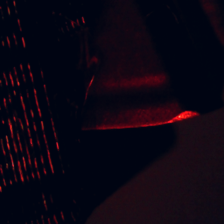
\includegraphics[width=\linewidth]{fig/results/wandb/spaghetti_dataset/images/media_images_Examples_r_128_p0_t2.png}
			\caption{Truth: Medium \\Predicted: High}
			\label{fig:res:sd:testimg:red:error}
		\end{subfigure}
		\hspace*{\fill}
		\begin{subfigure}{.24\textwidth}
			\centering
			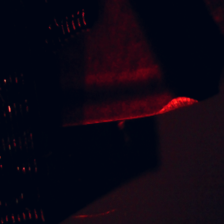
\includegraphics[width=\textwidth]{fig/results/wandb/spaghetti_dataset/images/media_images_Examples_r_96_p0_t0.png}
			\caption{Truth: High \\Predicted: High}
		\end{subfigure}
		\caption{Images with predictions from the spaghetti dataset with white lighting.}
		\label{fig:res:sd:testimg:red}
	\end{figure}


\section{Spaghetti dataset compared with second handmade dataset}
\label{sec:results:spaghettivsshm}
If we compare the results from the spaghetti dataset with the results that where obtained from the second handmade dataset, these results aren't as expected since the amount of data in the Spaghetti dataset is more than doubled but the results for the test are worse. To give an overview of the dataset three inserts are listed in Figure \ref{fig:res:comp:sd}:

\begin{itemize}
\item One from the second handmade dataset in Figure \ref{fig:res:comp:shd}
\item One from the white part of the Spaghetti dataset in Figure \ref{fig:res:comp:sd:white}
\item One from the red part of the Spaghetti dataset in Figure \ref{fig:res:comp:sd:red}
\end{itemize} 

	\begin{figure}[hbtp]
		\centering
		\begin{subfigure}{0.31\textwidth}
			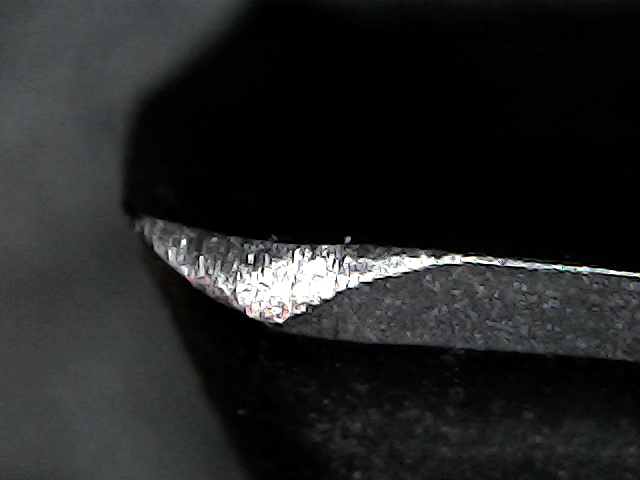
\includegraphics[width=\linewidth]{fig/Vision/Dataset/handmade_datasets/Second_handmade_dataset/b_005_p_010_s.jpg}
			\caption{Image from second handmade dataset}
			\label{fig:res:comp:shd}
		\end{subfigure}
		\hspace*{\fill}
		\begin{subfigure}{0.31\textwidth}
			\centering
			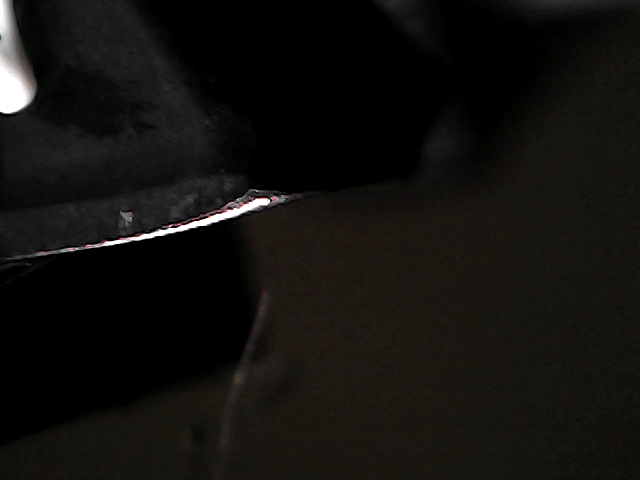
\includegraphics[width=\linewidth]{fig/Vision/Dataset/automated_datasets/2_created_datasets/2_Spaghetti_dataset/b_003_p_006_l_006-011_white_nb.png}
				\caption{Image from Spaghetti dataset white}
				\label{fig:res:comp:sd:white}
		\end{subfigure}
		\hspace*{\fill}
		\begin{subfigure}{0.31\textwidth}
			\centering
			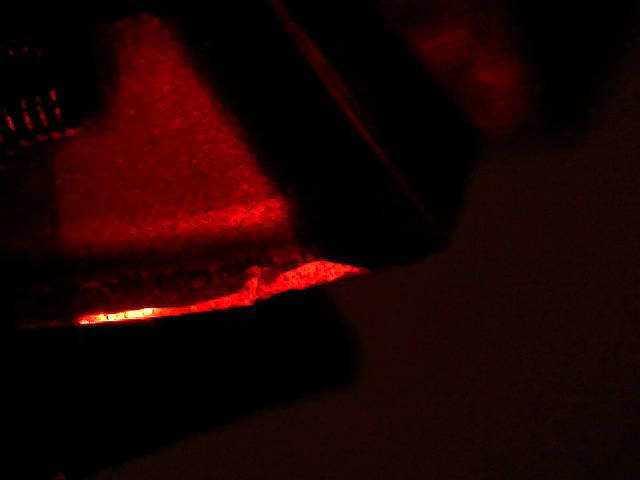
\includegraphics[width=\linewidth]{fig/Vision/Dataset/automated_datasets/2_created_datasets/2_Spaghetti_dataset/b_018_p_002_l_006-011_red_nb.png}
				\caption{Image from Spaghetti dataset red}
				\label{fig:res:comp:sd:red}
		\end{subfigure}
		\label{fig:res:comp:sd}
	\end{figure}
	
	For further investigation the datasets are globally compared first and after that the influence of the different model architectures on the datasets will be covered.

	\subsection{Global comparison}
	For this global comparison will the Spaghetti dataset be split up into a white and a red part so the results from the white part should match the results from the second handmade dataset. 
	
	First we compare the train accuracy and the validation accuracy to spot differences in the learning curve of these two datasets. For the training accuracy of Figure \ref{fig:res:comp:tra} we see that the second handmade dataset requires fewer training epochs and increases in train accuracy much quicker. For the validation accuracy in Figure \ref{fig:res:comp:va} there is a similar trend. 
	On both figures can be noticed that the standard deviation given in shadowed color is much larger for the Spaghetti dataset which means the training runs where much more fluctuating. 
	We can conclude from these results that the spaghetti dataset is much harder to learn. For the confirmation we look at Figure \ref{fig:res:comp:ta} where the test accuracy is plotted. The same conclusion can be extracted from this figure. The second handmade dataset has less fluctuation and produced much more consistent good results and the spaghetti dataset also reached an accuracy of 100\% but has much more runs with a lower accuracy. 

	\begin{figure}[hbtp]
		\begin{subfigure}{0.49\textwidth}
		\centering
		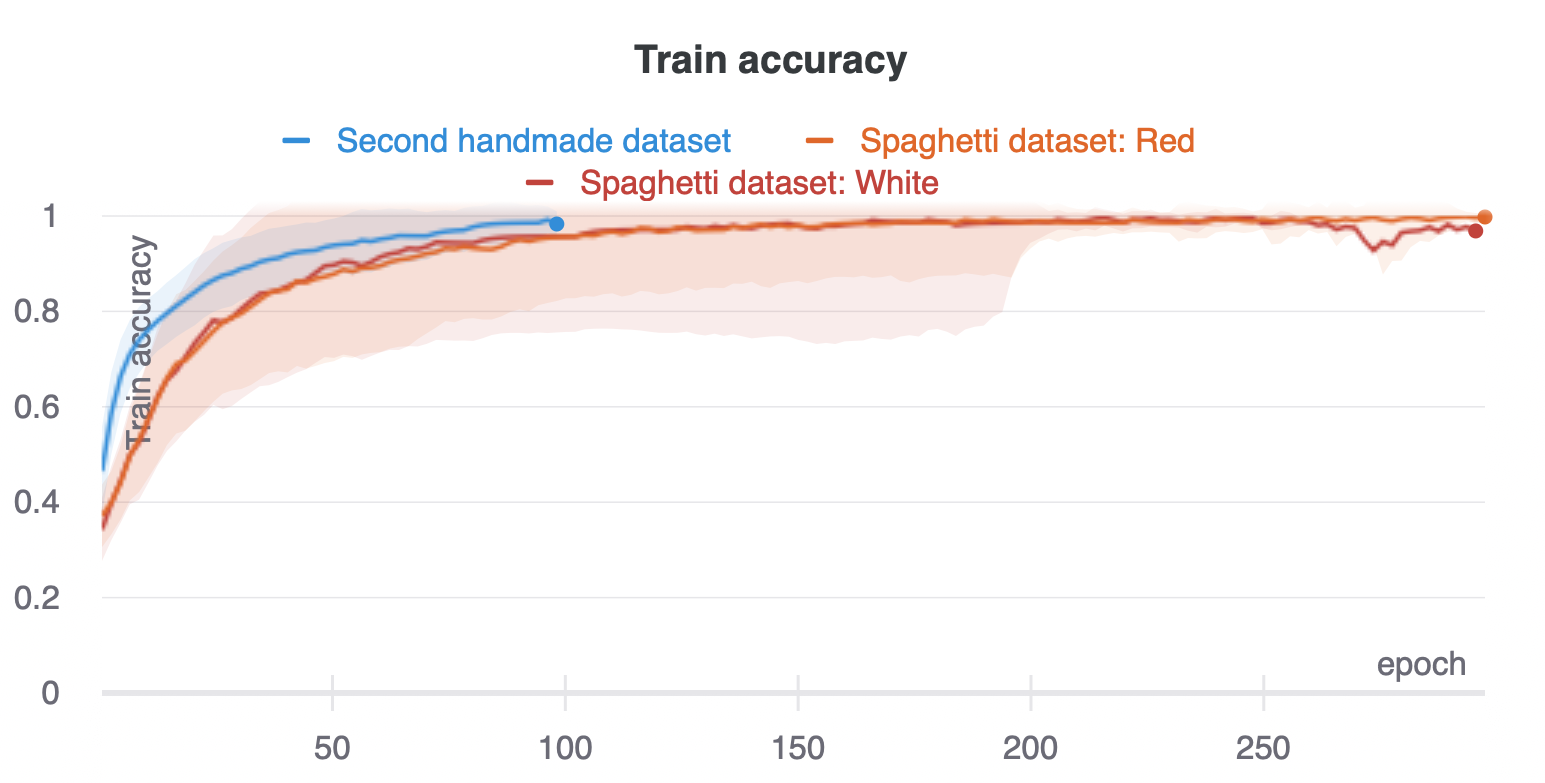
\includegraphics[width=\linewidth]{fig/results/wandb/spaghetti_vs_secondhandmade/charts/Section-2-Panel-0-d9vatkbok}
		\caption{Train accuracy}
		\label{fig:res:comp:tra}
		\end{subfigure}
		\hspace*{\fill}
		\begin{subfigure}{0.49\textwidth}
		\centering
		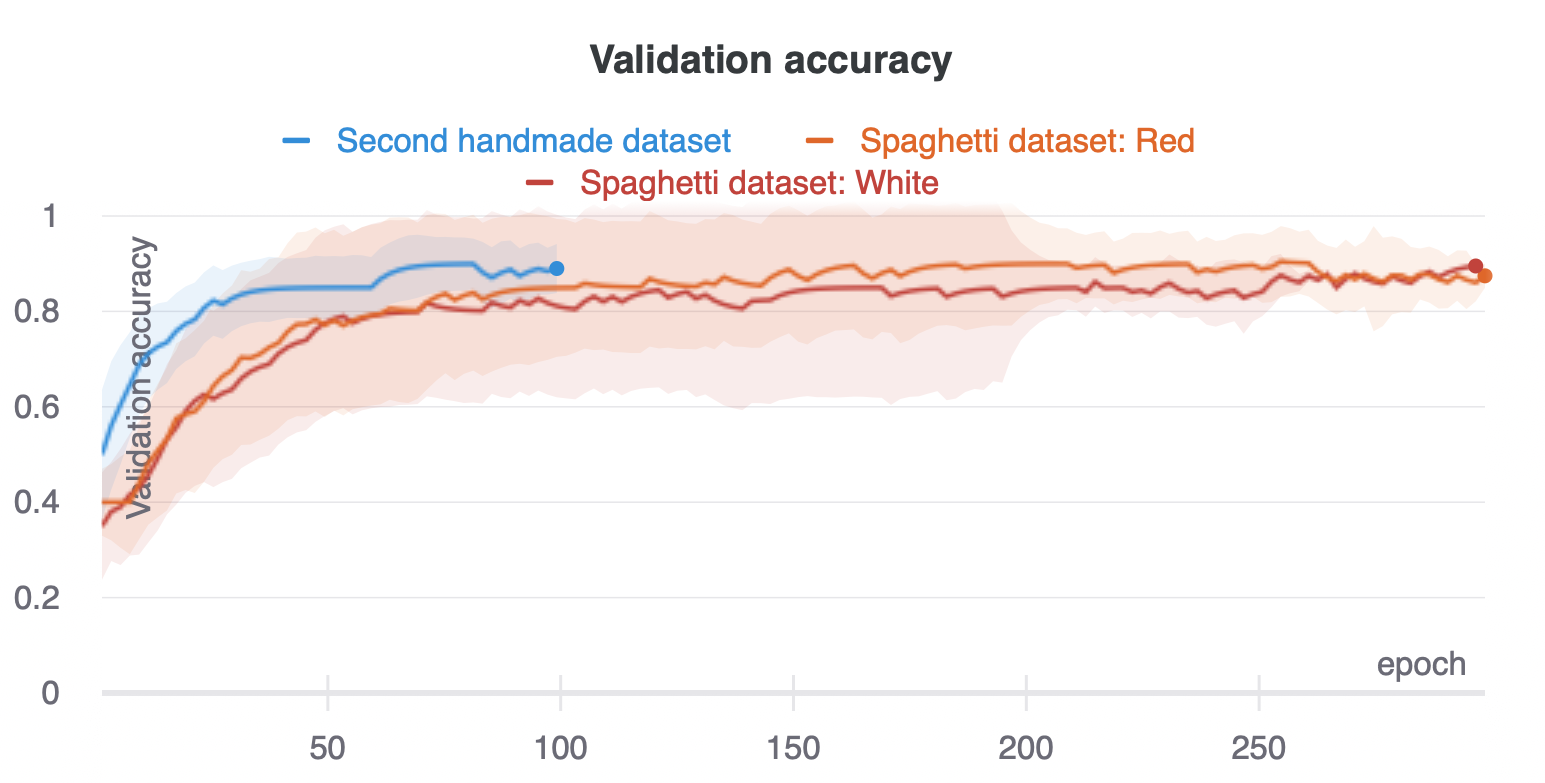
\includegraphics[width=\linewidth]{fig/results/wandb/spaghetti_vs_secondhandmade/charts/Section-2-Panel-1-h8kizzbrm}
		\caption{Validation accuracy}
		\label{fig:res:comp:va}
		\end{subfigure}
		\hspace*{\fill}
		\begin{subfigure}{0.6\textwidth}
		\centering
		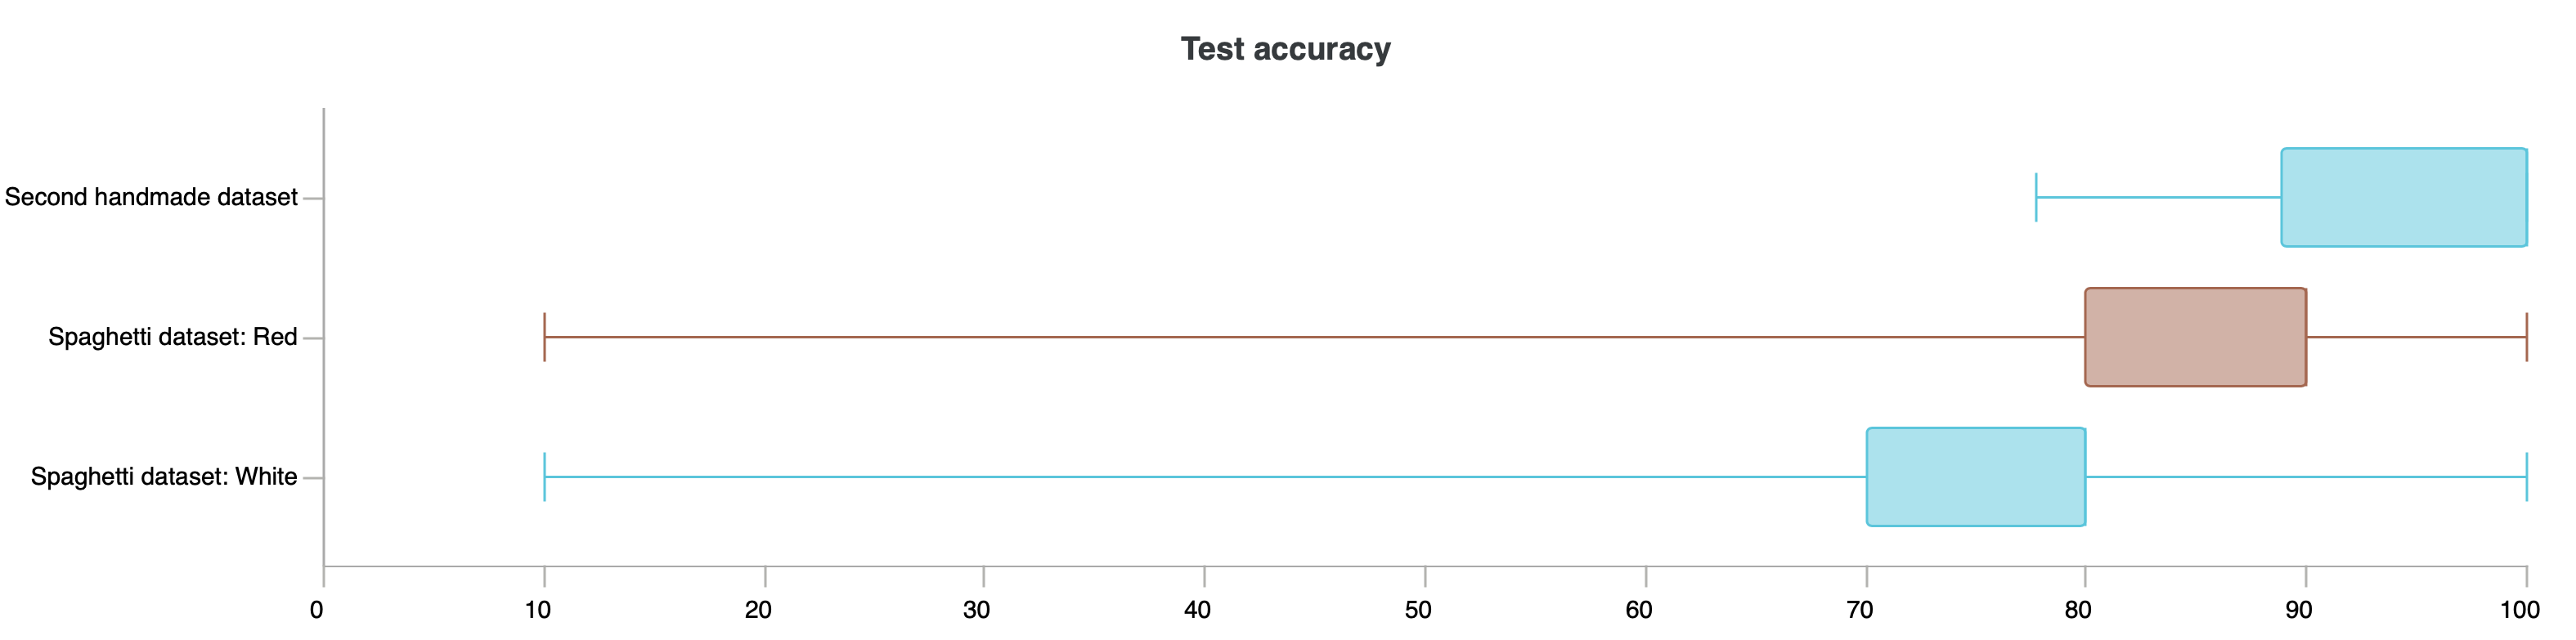
\includegraphics[width=\linewidth]{fig/results/wandb/spaghetti_vs_secondhandmade/charts/Section-2-Panel-2-mwwjkupji}
		\caption{Test accuracy}
		\label{fig:res:comp:ta}
		\end{subfigure}
		\hspace*{\fill}
		\caption{Comparison for test, train and validation accuracy for different datasets.}
		\label{fig:res:comp}
	\end{figure}
	
	Table \ref{tab:results:comparison:valacc} shows the validation accuracy for the white part of the Spaghetti dataset. These results can be compared with the results from the second handmade dataset in table \ref{tab:results:shm:architectures:valacc}. The same order is kept and even the values don't differ much. Alexnet, Resnet 18 and Squeezenet can be said to be the best architectures for this problem with a smaller, simpler dataset.
	This table can also be compared against table \ref{tab:results:spaghetti:valacc} from the full spaghetti dataset where the order is basically reversed. 
	
	This observation can be declared based on the Table \ref{tab:lit:ov:paramdepth} 
	Alexnet, Resnet 18 and Squeezenet all have similar values for the number of parameters and depth (61.1 M, 11.7 M, 1.2 M) and (8, 18, 10) respectively. VGG11 has 123.1 M parameters and 11 layers and Densenet 121 has 7.9 M parameters and 121 layers. From this information we can conclude that a wider network with less parameters and layers produces better results for this easy problem with a small dataset. 
	But for the more difficult problem with the Spaghetti dataset where more data is provided, the architectures with more parameters and layers like VGG11 and Densenet 121 are better. 
	
	\begin{table}[!ht]
		\centering
		\caption{Validation accuracy for the white part of the Spaghetti dataset. First column is sorted on best validation accuracy, second column is sorted on best Test accuracy.}
		\begin{tabular}{ c | c c }
			%\caption{Confusion matrix for tests of Second handmade dataset}
			Model name		& Validation Accuracy 	& Validation accuracy sorted on test accuracy	\\ \hline
			Alexnet			& 100\%							& 100\%					\\
			Resnet 18 		& 100\%						& 100\%					\\
		 	Squeezenet			& 100\%							& 100\%					\\
			VGG11\_bn 			& 90\%						& 90\%					\\
		 	Densenet 				& 90\%						& 90\% 				\\ 
		\end{tabular}
		\label{tab:results:comparison:valacc}
	\end{table}
		
\subsection{difference for different model architectures}

	To check the influence of the model architecture on the dataset we plot the test accuracy for every dataset and all different architectures. This is shown in Figure \ref{fig:res:comp:ta:arch} where SHM stands for second handmade dataset; red stands for the red part of the spaghetti dataset and white for the white part.
	
	The same conclusions can be made for these models as for the global results for these datasets. The model architecture doesn't incorporate a sufficient difference in results. 

	\begin{figure}[hbtp]
		\centering
		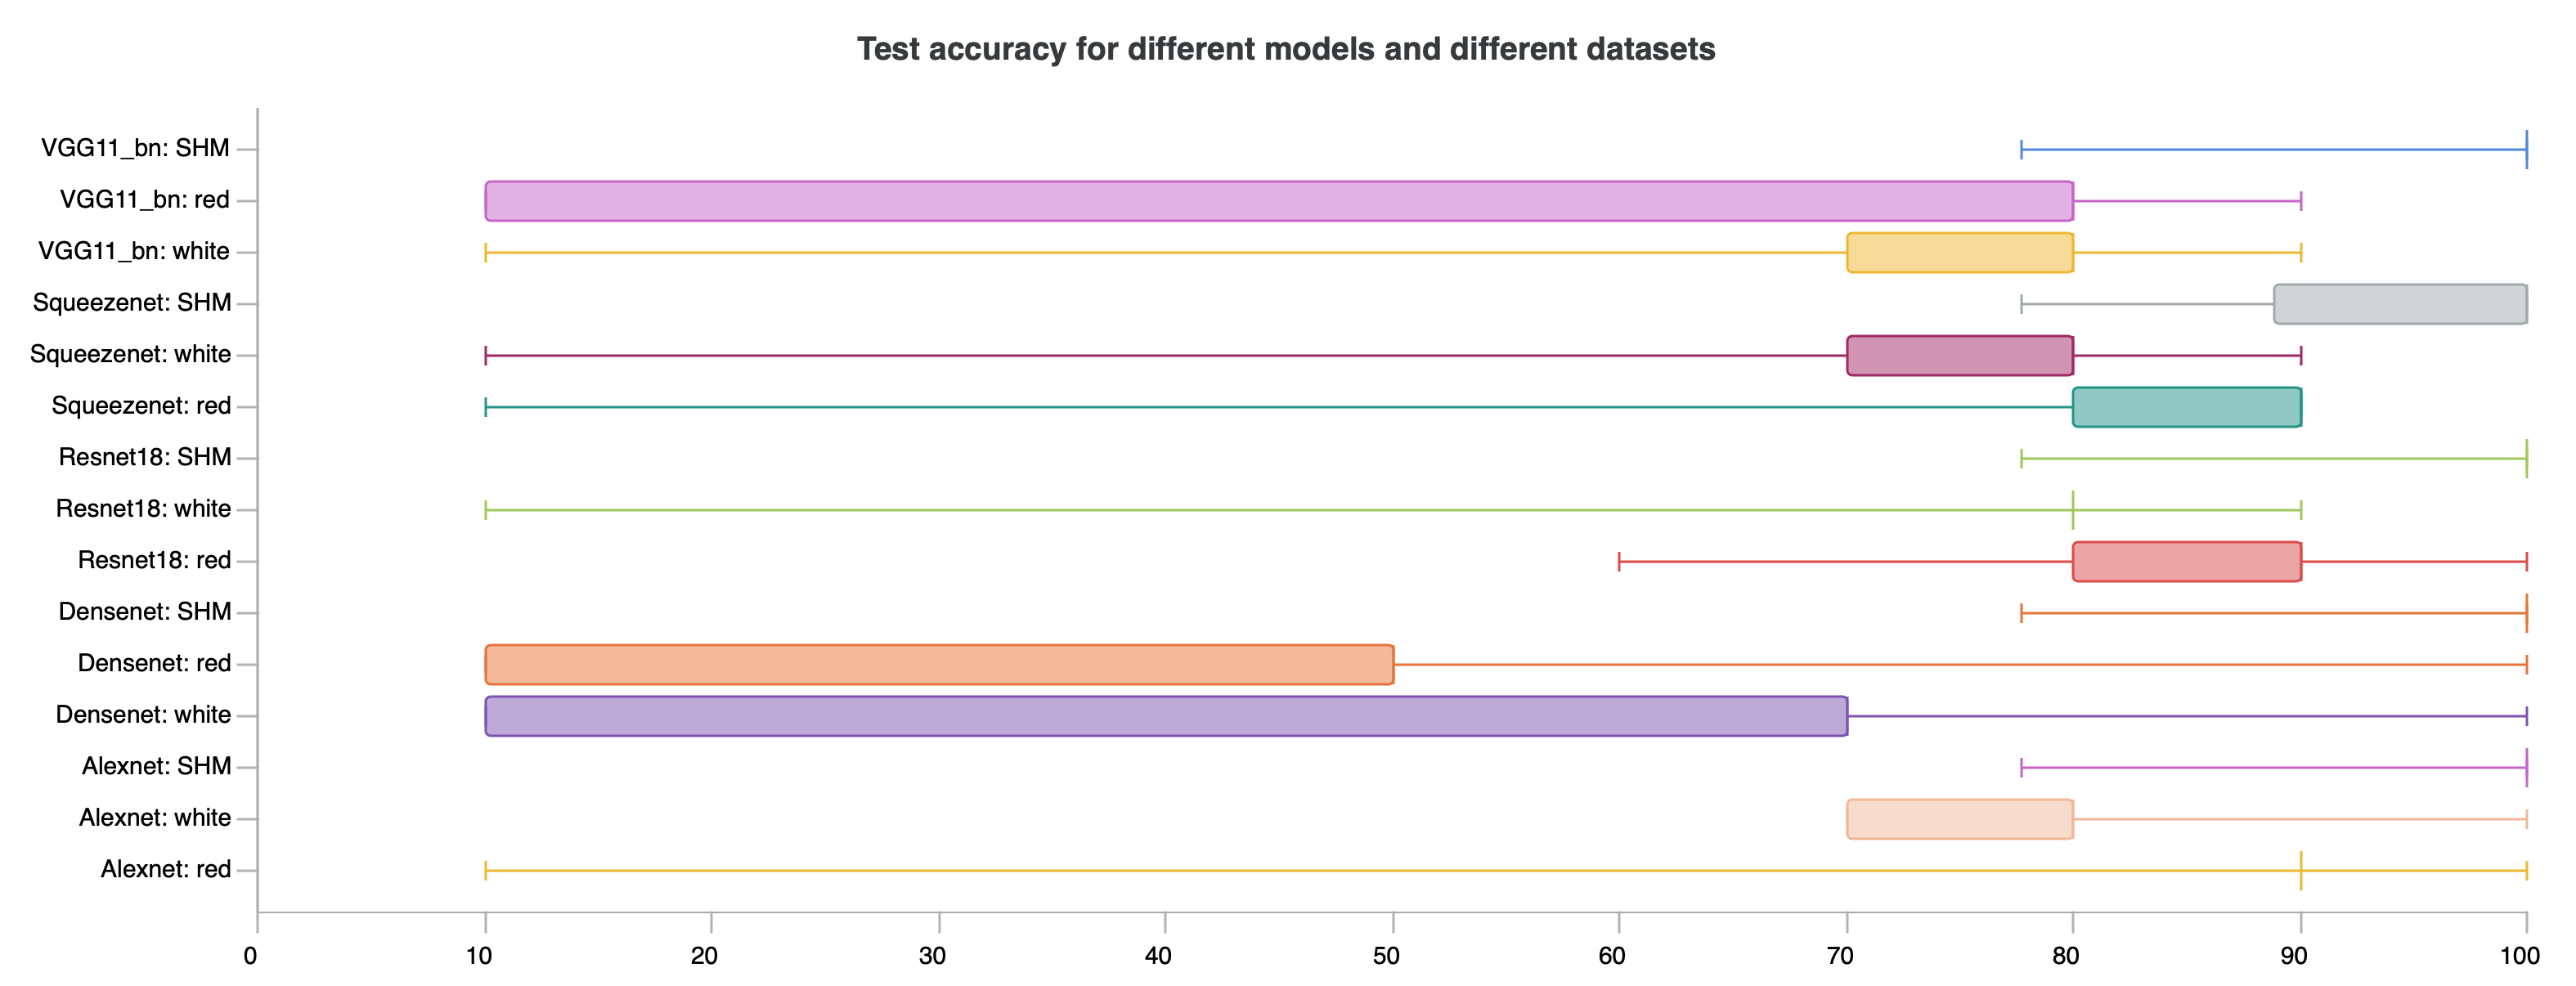
\includegraphics[width=\linewidth]{fig/results/wandb/spaghetti_vs_secondhandmade/charts/Section-4-Panel-0-u37bm4h79}
		\caption{Difference in test accuracy for different datasets trained with different model architectures.}
		\label{fig:res:comp:ta:arch}
	\end{figure}

As already noted in the section about the spaghetti dataset, there are disturbances in the images where the white or black plastic from the tool holder comes into the frame. This makes it harder to separate some pictures. Secondly the position of the worn area isn't always the same like in the second handmade dataset. 

To conclude: the images must be taken a bit better so less unwanted things are in the picture and the wear should be lightened in a way that makes it possible to detect the different wear areas on different inserts.

